\documentclass[11.5pt]{article}
\usepackage[table]{xcolor}
\definecolor{lightgray}{gray}{0.9}
\usepackage{multirow} 
\usepackage{lscape}
\usepackage{filecontents}
\usepackage[left=2.5cm,top=2.5cm,right=2.5cm,bottom=2.5cm]{geometry}
\usepackage{amsmath}
\usepackage{array}
\usepackage{caption}
\usepackage{longtable}
\usepackage{placeins}
\usepackage{graphicx}
\usepackage{subcaption}
\usepackage{setspace}
\usepackage{animate}
%\usepackage[active,tightpage]{preview}
\usepackage{natbib}
\bibpunct{(}{)}{,}{a}{}{;} 
\usepackage{url}
\usepackage{nth}
\usepackage{authblk}
\usepackage{listings}
% for the d in integrals
\newcommand{\dd}{\; \mathrm{d}}
\newcommand{\tc}{\quad\quad\text{,}}
\newcommand{\tp}{\quad\quad\text{.}}
\bibliographystyle{apalike}

\title{ Deviations in avoidable causes of death in adulthood drive mortality inequality between
Mexican states}

%\author[1]{Nancy Plascencia\thanks{nancy.plascemcia@agricomer.com}}
\author[1]{Jos\'e Manuel Aburto}
%\author[3]{Ainhoa Alustiza}
\author[2]{Tim Riffe}
\affil[1]{European Doctoral School of Demography}
\affil[1,2]{Max Planck Institute for Demographic Research}


\begin{document}

\maketitle

\begin{abstract}
We analyze trends in temporary life expectancy for three large age groups from 1990 to 2015 for all 32 Mexican states, and compare these with a low mortality benchmark. We assess the impact of avoidable/amenable mortality on temporary life expectancy at the state level by sex. We apply demographic measures and use standard decomposition techniques to disentangle the effects of selected causes of death on trends in state health inequality. We find improvements in temporary life expectancy for the population aged 0 to 14, as they continuously approached the low mortality benchmark. However, the adult population aged 15 to 39 shows deterioration among males after 2006 in almost every state. Females on the whole converged toward the low mortality benchmark in the same age group. Adults aged 40 to 74 show an unexpected decrease in the mow mortality benchmark, indicating universal deterioration in temporary life expectancy for this age group, albeit with wide variation between states. These findings support the case for reforms that treat all causes of death as public health priorities, and that target regional disparities in health.

\end{abstract}

\section*{Key messages}
\begin{itemize}
\item Reducing health inequalities among sub-populations is a goal of every developing country. Addressing such inequalities in older adult populations in Mexico is proving to be a challenge to reaching this goal.
\item We hypothesize age-dependent variations in temporary life expectancy between states. Particularly due to the rise in homicide mortality and the increase of conditions amenable to medical services and policy/behavior actions.
\item Our results show that deviations from our low mortality benchmark are mainly driven by adult mortality. Young-age mortality has steadily converged toward the low mortality benchmark, pointing towards the success of public health interventions.
\item Cirrhosis, homicide, diabetes and isquemic heart diseases contribute the most to the persistence of health inequalities between Mexican states. Importantly, some of them could gain up to two years of life on average if the low mortality benchmark were achieved.
\end{itemize}

\begin{spacing}{1.5}
\section*{Introduction (max 6000 words)}
The \nth{20} century was marked by sizable improvements in mortality, living
conditions and health in most Latin American countries \citep{who2000}. 
In Mexico, these improvements have slowed down recently as a result of opposing
trends in particular causes of death. For instance, homicide and diabetes
increased dramatically, even as infectious and
respiratory diseases continued to fall. While life
expectancy at birth increased by 4.3 years for males (from 67.6 to 71.9) and 3.4
for females (from 73.8 to 77.2) between 1990 and 2000 \citep{SOMEDE},
between 2000 and 2010, life expectancy at birth entered into a period of
stagnation for males and slowed progress for females \citep{canudas2014}. 


This
period coincides with the implementation of different public health
interventions, such as the Universal Vaccination Program and Seguro
Popular, which aim to provide primary and secondary
health care to the uninsured population and allocate funds to cover catastrophic
health expenditures \citep{knaul2005}. Further, the conditional cash transfer program PROGRESA/Oportunidades
was introduced to supply incentives for families to invest in themselves and
benefit from education, health, and nutrition in the late 1990's \citep{neufeld2012}. Some evidence
suggests that Mexico experienced substantial decreases in infant and child
mortality, along with improvements that contributed to the reduction of
mortality and in the prevalence of acute malnutrition between 1980 and 2000
because of these interventions \citep{sepulveda2006}. Similarly, some evidence
suggests that by 2012 Seguro Popular had covered an additional 52 million
people in Mexico that did not have any access to public health care and, as a result, there has been a reduction in catastrophic health expenditures \citep{knaul2012}.

These results underscore the progress in public health interventions, but they do not reveal heterogeneity between Mexican states or the epidemiological patterns for different age groups. Given improvements in health care coverage, the strong role of institutions, and ongoing public
 health interventions, it is necessary to assess the varied impacts that
 these interventions may have had on mortality on Mexican states. For instance, PROGRESA/Oportunidades is focused on the poorest states, and Seguro Popular was introduced at different times in different states. In addition, the high degree of social and health inequalities present in the country \citep{Frenk2006} support this task as Mexico faces a rapid ageing process -the percentage of the population aged 60 or older will go from 10\% in 2015 to 15\% in 2030  \citep{CONAPO}- in which the interaction between infectious diseases and noncommunicable conditions, such as diabetes, is anticipated and must be considered from a public health perspective \citep{Bygbjerg1499}. Identifying specific opportunities to improve and put forward solutions to reduce the gap of  the unequal impact of public health interventions on population's health is a necessary step to increase survival among the Mexican population.
 
 One approach to assess the impact of health care and other interventions is by operationalizing the
 concept of Avoidable/Amenable Mortality (hereafter abbreviated AM)
 \citep{nolte&mckee2004, nolte&mckee2008,elo2014}. This construct aims to measure the quality of health service systems by selecting certain
 causes of death that should not occur in the presence of effective and
 timely health care. Among industrialized countries (e.g., United States,
 Australia, France, Japan), a reduction in AM rates was
 observed from the late 1990's into the \nth{21} Century
 \citep{nolte&mckee2008}. Avoidable mortality rates fell, on average, by 17\%
 for males and 14\% for females in these countries. Despite mortality reductions for
 both sexes, heterogeneity between countries was identified, with the United
 States showing the smallest reductions (around 5\%) for both sexes. However,
 each country showed progress in mortality from treatable cancers and
 circulatory diseases except for ischemic heart diseases.

In Mexico, the components of avoidable mortality had different trends since the
late 1990's. Between 2000 and 2004 AM decreased, particularly from
infectious diseases and nutrition-related conditions \citep{francomarina2006}, while it increased between 1998 and 2010 due to diabetes, circulatory diseases, perinatal and respiratory conditions
\citep{agudelo2014efecto}. Increases in the latter causes
of death were particularly concentrated in the poorest states of the country
\citep{davila2014mortalidad}. We aim to extend these studies
by a more focused segmentation of AM into health intervention-related AM and
behavior-related AM. Also, we extend analysis to all 32 states, by sex, and over
the full 26-year period from 1990 to 2015. Finally, we compare state mortality patterns
with an easy-to-understand low-mortality benchmark calculated for large age groups (e.g., 0-14, 15-39, 40-75). This low mortality
benchmarks is calculated on the basis of the lowest observed mortality within
ages and causes, selected from the full set of 32 Mexican states. This concept was first
proposed by \citet{whelpton1947}, later explored by  \citet{wunsch1975minimum} and
\citet{vallin2008minimum}. Deviations from the low-mortality benchmark indicate a strong potential for improvement. We apply demographic measures and
standard decomposition techniques to isolate the cause and age-specific deviations between states and the corresponding optimal lifetable. 

We hypothesize age-dependent variations in temporary life expectancy outcomes.
In particular, we expect convergence between states in temporary life expectancy
for young people, since public health interventions are mainly focused in infant
mortality and child health . For instance, the vaccination program and the health
reform aim to fully cover children in the entire country, and recent
evidence suggests a decrease in mortality between ages 0 to 14 due to a decline
in infectious and respiratory diseases \citep{canudas2014}. On the contrary, we
expect little improvements in temporary life expectancy for the adult and older
adult population due to the unprecedented rise in homicide mortality and the
increase in diabetes mortality along with endocrine/metabolic diseases in these ages in the country \citep{canudas2014}. Although every
state has the commitment to providing universal coverage and equitable access to
health care since the early 2000's, we anticipate heterogeneity between states
in mortality improvements due to state differences in epidemiological patterns and the differential in how benefits of health care programs have been delivered to the population
\citep{Frenk2006}.


\section*{Data \& Methods} 
Our analyses are based on publicly available anonymized datasets. We used deaths microdata available from official files produced by the
Mexican Statistical Office from 1990 to 2015 \citep{INEGI}. These data contain necessary
information on causes of death by single age, sex, and state of residence at the
time of death. Population estimates from 1990 to 2010 came from the Mexican Society of Demography. These estimates adjust for age misstatement, undercounting, and interstate and international migration. Additionally, we estimate intercensal population counts by age, sex and state for the period 2011-2014 using the most recent inter-census survey that tool place in 2015  \citep{INEGI}. Death counts and population exposures were used to calculate cause-age-specific death rates by sex and state from 1990 to 2014.

\subsection*{Classification of Causes of Death}

To separate causes of death that are susceptible to medical intervention (e.g.,
infectious and respiratory diseases) and those related to health behaviors and
intersectoral policies (e.g., homicides, lung cancer) we use the concept of
'Avoidable/Amenable Mortality' (AM) \citep{nolte&mckee2004, nolte&mckee2008}. This
concept assumes a list of conditions that should not cause death if timely medical care is available. Recently, this concept has also been used to gauge the
effect of causes that can be influenced by public policy (e.g., cirrhosis) \citep{elo2014}. We classified causes of death into ten groups based on prior studies , as listed in Table~\ref{tab:causes}, with
relative frequencies by sex \citep{elo2014, Aburto2015}.

% latex table generated in R 3.2.2 by xtable 1.8-0 package
% Mon Feb  8 21:50:32 2016
% latex table generated in R 3.2.2 by xtable 1.8-0 package
% Mon Feb  8 21:52:20 2016
\begin{table}[ht]
\centering
\caption{Avoidable Mortality classification, 
             with crude percentages below age 75.} 
\label{tab:causes}
\begin{tabular}{lllll}
  \hline
Category &\% & Males &  \% & Females \\ 
  \hline
Causes amenable to medical service &                             28.5 \% &                          1,130,574 &                            40.24 \% &                          1,067,159 \\ 
                            Diabetes &                             9.07 \% &                            359,947 &                            14.77 \% &                            391,760 \\ 
             Ischemic heart diseases &                             7.92 \% &                            314,312 &                             6.66 \% &                            176,734 \\ 
                            HIV/AIDS &                              1.8 \% &                             71,536 &                             0.51 \% &                             13,564 \\ 
                         Lung cancer &                             1.58 \% &                             62,532 &                             1.09 \% &                             28,895 \\ 
                           Cirrhosis &                             5.34 \% &                            212,035 &                             1.09 \% &                             28,999 \\ 
                            Homicide &                             5.95 \% &                            236,152 &                             1.05 \% &                             27,802 \\ 
              Road traffic accidents &                             5.82 \% &                            231,045 &                             2.26 \% &                             59,967 \\ 
                             Suicide &                             1.48 \% &                             58,683 &                             0.46 \% &                             12,131 \\ 
                        Other causes &                            32.53 \% &                          1,290,596 &                            31.86 \% &                            844,963 \\ 
   \hline
\end{tabular}
\end{table}

% latex table generated in R 3.1.2 by xtable 1.7-4 package
% Wed Sep 23 21:57:18 2015
%\begin{table}[ht]
%\centering
%\caption{Avoidable Mortality classification, with crude percentages below age 75.}
%\label{tab:causes}
%\begin{tabular}{>{\raggedright}m{3cm}rr}
%Group/Cause  & Males & Females \\ 
%  \hline
%Causes amenable to medical service & 28.50 & 40.24 \\ 
%  Diabetes & 9.07 & 14.77 \\ 
%  Ischemic heart diseases & 7.92 & 6.66 \\ 
%  HIV/AIDS & 1.80 & 0.51 \\ 
%  Lung cancer & 1.58 & 1.09 \\ 
%  Cirrhosis & 5.34 & 1.09 \\ 
%  Homicide & 5.95 & 1.05 \\ 
%  Road traffic accidents & 5.82 & 2.26 \\ 
%  Suicide & 1.48 & 0.46 \\ 
%  Other causes & 32.53 & 31.86 \\ 
%   \hline
%\end{tabular}
%\end{table}

We separate diabetes, ischemic heart diseases (IHD), HIV/AIDS, lung
cancer, and cirrhosis because all of them are amenable to both health behavior
and medical service, and because the first two represent major causes of death
in Mexico \citep{canudas2014}. In addition to these causes, we also separate
homicide, road traffic accidents, and suicide because they have emerged as
leading causes of death among young people, and the first two had a sizeable
impact on life expectancy recently in Mexico \citep{canudas2014}. All causes of death were classified using the International Classification of Diseases, revision 9 for the period 1990-1997 and the tenth revision for 1998-2015 (see Appendix Table 1 for details on ICD codes for each cause).

We truncated analysis at age 75 because classification of causes of deaths and age reporting are considered to be innacurate in death registration at older ages \citep{tobias2001}. Most changes in life expectancy are likely due to changes in mortality patterns below the age of 75 \citep{Aburto2015}. In addition, health care and policy/behavior interventions are more likely to be effective at younger ages \citep{elo2014}.

\subsection*{Age dimension}

We break life expectancy in three large age groups to capture mortality differences along the lifespan based on previous research. The first group, young people, refers to people younger than 15 years. This group (0-14) is likely to represent improvements in causes amenable to medical service (e.g. infectious diseases and conditions of perinatal period) \citep{canudas2014}. The second group, young adults, allude to the population aged 15-39. We use this interval in order to capture the effect of homicide mortality and external causes, which have an important impact on life expectancy in these ages \citep{Aburto2015}. Finally, the third group, older-adults, makes reference to the population older than 40 years up to 75. The population in this group represents the core of this article and they are susceptible of experiencing premature death due to chronic diseases \citep{canudas2014}.


\subsection*{Demographic Methods}
We smooth cause-specific death rates over age and time for each
state and sex separately using the 2-d p-spline method proposed by
\citet{GC2012}.
This helps eliminate stochastic zeros, which otherwise would accumulate in minimum mortality
schedule. Smoothed death rates are
then constrained to sum to the unsmoothed all-cause death rates. We then calculate period life tables up to
age 74 for males and females from 1990 to 2010 following the HMD Methods
Protocol \citep{HMDMP}. We calculate temporary life expectancy to
capture differential effects of all-cause mortality in three large age
groups: children (ages 0-14), young adults (ages 15-40) and older adults
(40-74).

We estimate cause-specific contributions to the difference between
state-specific temporary life expectancy and benchmark temporary life expectancy
($e^{\star}$) applying standard decomposition methods
\citep{horiuchi2008}. Decomposition techniques are a suitable method for comparing life expectancies across populations and analyzing age and cause-specific contributions to their differences \citep{preston2001}. All the analyses were carried out
using \texttt{R}.

\subsection*{Low mortality benchmark}
This approach was first proposed by \citet{whelpton1947}, and we summarize it
briefly here. The low mortality lifetable is bases on synthetic mortality rates, defined as the sum of the lowest observed mortality rates by age, cause,from among all states for a given sex and year. The low mortality rates $\mu(x)^\star$, are calculated as the sum of $C$ cause-specific minimum mortality rates at age $x$, under the assumption that causes of deatg are independent of one another:
\begin{equation}
\label{eq:mxmin}
\mu(x)^{\star} = \sum_c=1^C min(\mu(x,c,s))
\end{equation}

where $x$ is age, $c$ is the given cause of death, and $s$ indexes the set of 32 states from which the minimum is selected. The resulting minimum mortality rate schedule $(\mu(x)^{\star})$ has a unique age profile, and it determines our benchmark life expectancy, $e(0)^\star$. $e(0)^\star$ can be treated as the maximum presently achievable life expectancy assuming perfect diffusion of the best available practices and technologies within a given set of populations, \citep{vallin2008minimum}. It is an imaginary quantity because no particular population is expected to achieve this mortality pattern. However, this value is a practical reference because it is based neither on a projection of improvements into the future nor on an arbitrary and likely dissimilar population. We refer to the state with the highest life expectancy in a given year as the vanguard state. 



\subsection*{Temporary Life Expectancy}

Temporary life expectancy between ages
$x_1$ and $x_2$, for $x_1<x_2$, is defined as the average years of life lived between these ages according to a given set of mortality rates \citep{arriaga1984}. We denote this quantity as
$e(x_1,x_2)$, and its benchmark minimum as $e^{\star}(x_1,x_2)$. Defined in
terms of lifetable survivorship, $\ell(x)$:

\begin{equation}
e(x_1,x_2) = \frac{\int _{x_1}^{x_2} \ell(x) \dd x}{\ell(x_1)}
\end{equation}

The interpretation of temporary life expectancy has the advantage, that if nobody dies between the starting and ending age, then the maximum life expectancy is $x_2-x_1$.  For example, if we set $x_1=0$ and $x_2=14$, if no person dies between the ages 0 and 14, on average the population lives 14 full years, which means that the temporary life expectancy between these ages, $e(0,14)$, is fourteen. Which sets a maximum achievable and, therefore, measurable.

\subsection*{Limitations}
The limitations of our study should be mentioned. First, mortality data are
likely to present inaccuracies in cause-of-death classification due to
comorbidities, particularly at older ages \citep{tobias2001}. To mitigate this,
we focus on ages below 75, grouping causes of death using ICD codes according to
the avoidable mortality concept.
Second, our estimates regarding homicide mortality are likely to be
underestimated because of inaccurate practices regarding counting, reporting,
and due to the large number of missing individuals in Mexico \citep{HRW2011}.
Third, avoidable mortality should be understood as an indicator of potential
weaknesses with respect to health care and some public health policies and not
as a definitive assessment \citep{nolte&mckee2008}. Fourth, the amount of deaths
that should be considered avoidable within the avoidable classification is not
clear \citep{beltran2011avoidable}. For instance, \citet{nolte2012amenable}
consider only 50 percent of heart disease amenable in industrialized countries,
based on a previous review of evidence.

We do not have information to precisely
measure percentages of avoidable mortality within cause groups. Nonetheless, the
difference between a given mortality schedule and the best practices schedule of
the same year can be conceived of as a minimal definition of avoidable
mortality. A sort of lower bound to how much mortality could have been avoided.
Certainly, even a best practices schedule will contain elements of mortality
most would consider avoidable. To the extent that the components of the benchmark schedule were indeed
attained somewhere in the population universe, one can view any excess mortality
with respect to the benchmark schedule as avoidable. Little progress has been made in advancing the concept of avoidable mortality \citep{holland2003}. We believe this perspective improves on the original concept and gauge better the avoidable deaths.

\section*{Results}
\subsection*{Trends in low mortality benchmark and temporary life expectancy}
Figure 1 presents the state-specific trends in temporary life expectancy for young, young-adult and older-adult populations (black lines). The red lines represents the record holder state in a given year, while the blue line is related to the low mortality benchmark, which represents the maximum achievable survival for any state. Panel a) shows the convergence pattern among the young population. Since the 1990's all the states have shown improvements towards the low mortality benchmark, approaching near-complete survival between ages 0 and 14. However, some states (e.g. Puebla, Tlaxcala and M\'exico state) have lagged behind relative to the rest of states. The same pattern is observed in both females and males. 

Opposing this trend, temporary life expectancy between 15 and 39 years shows a common shift after 2005 in almost every state in Mexico  (panel b)). Some states (e.g. Chihuahua, Sinaloa in the northern region) experienced a dramatic deterioration that led to a potential increase of over two years on survival by 2010 between these ages.  Over the full period Oaxaca in the south, Baja California and Chihuahua from the north show the largest disparities relative to the low mortality benchmark. Results for females show stagnation, as in males' results, some states experienced losses of life after 2005, leading to widening the gap between states and the low mortality benchmark. However, females experience almost a full survival between ages 15 and 39 throughout the entire period. 


Temporary life expectancy for adults between 40 and 75 years shows stagnation and deterioration during the entire period (panel c)). Even the low mortality benchmark exhibits a downward trend, pointing to increases in adult mortality. In perspective, out of full-34 potentially livable years, all the states are living less than 30 years on average for males and 32 for females. Importantly, the lowest states (Baja California, Chihuahua and Sonora) could potentially leave more than two additional years if the low mortality benchmark were achieved. Similar to the young-adult males some states experienced a  clear downward after 2005. Results for females, show stagnation on the full survival in this age-group. 

These results show the mortality inequality prevalent in Mexico over the last 25 years by state, sex and age-groups. They also allow us to identify three very different patterns among the age groups and states. Young mortality has been decreasing approaching almost complete survival between ages 0-14. Young adults, particularly males, present a clear reversal in temporary life expectancy after 2005. While older adults show, both females and males, stagnation and deterioration since the 1990's leading to potential gains in life expectancy if survival between 40 and 75 is improved. To fully understand the underlying causes of death driving these stories, we decompose the gap between state-specific temporary life expectancy and the low mortality benchmark within each age-group.


\begin{figure}
\label{Fig_temporary_le}
\centering
\caption{Temporary life expectancy for states (black line), record life
expectancy (red) and low mortality benchmark by sex, 1990-2015.}
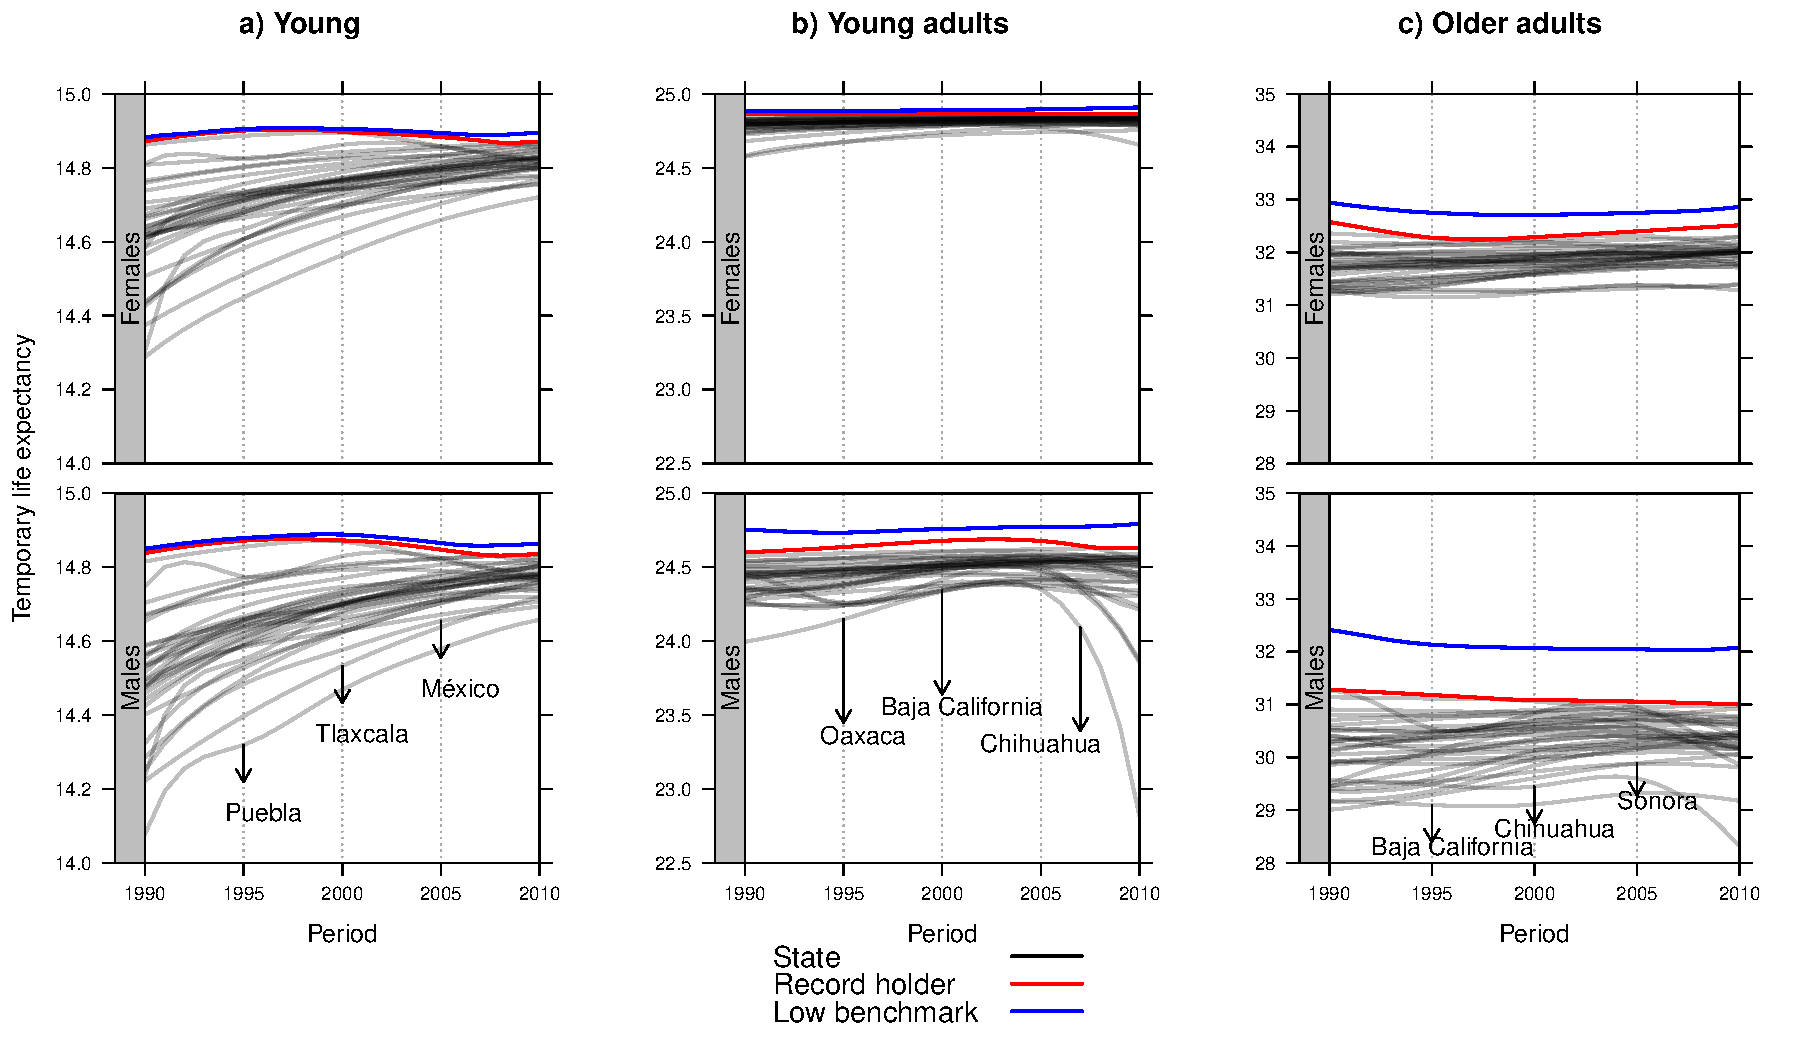
\includegraphics[scale=.5]{Figures/Temp_fig.pdf}

Note: Y-axis are not in the same scale in order to capture major trends over the period. Source: own calculations based on INEGI and SOMEDE files. 
\end{figure}

%\FloatBarrier
%\subsection*{State trends in departures from best practices temp e(0)}
%Small multiples maps (time series of maps)


\subsection*{Cause-decomposition analysis \footnote{This section will be completed at a later date and updated to 2015. Preliminary results are shown.
}}

Adult mortality shows the largest deviations from the low mortality benchmark compared with the other age-groups. Figures  \ref{fig:e40_74_females} and \ref{fig:e40_74_males} show cause-specific contributions to the gap between observed temporary life expectancy and the low mortality benchmark by state and region for females and males, respectively. Light-yellow colors indicate no contributions to the gap, which means that are very close to the low mortality benchmark within each category. Darker yellow and red colors indicate larger contributions to the gap. If a particular state is improving during the period, we expect a transition from red to light-yellow. 

As shown in figure \ref{fig:e40_74_females}, medically amenable causes of death still contribute to the gap between survival and the low mortality benchmark. However, improvements in this category throughout the period 1990-2015 helped deviations to get smaller in almost every state. Chihuahua, Coahuila and Baja California, in the northern region, and Chiapas in the south exhibit the largest deviations from the low mortality benchmark as female-mortality due to these causes stagnated. Opposing this, the increase of diabetes mortality among women has contributed to widening the gap between temporary life expectancy and the low mortality benchmark. Some states, like Tabasco in the south and Coahuila in the north, show a clear deterioration on the survival in the 2000's due to this cause of death. Isquemic heart diseases (IHD) is the the third cause of death that contribute the most to mortality inequality among regions. The impact of IHD on the survival of the adult-female population is concentrated in the northern region, as they have remain steady since the early 1990's. The rest of AM-categories do not contribute significantly to the gap between female survival and the low mortality benchmark, which means that they are very close to the latter.

\begin{figure}[h]
\centering
\caption{Cause-specific contributions to state differences from low mortality benchmark for older female adults, 1990-2015.}
\label{fig:e40_74_females}
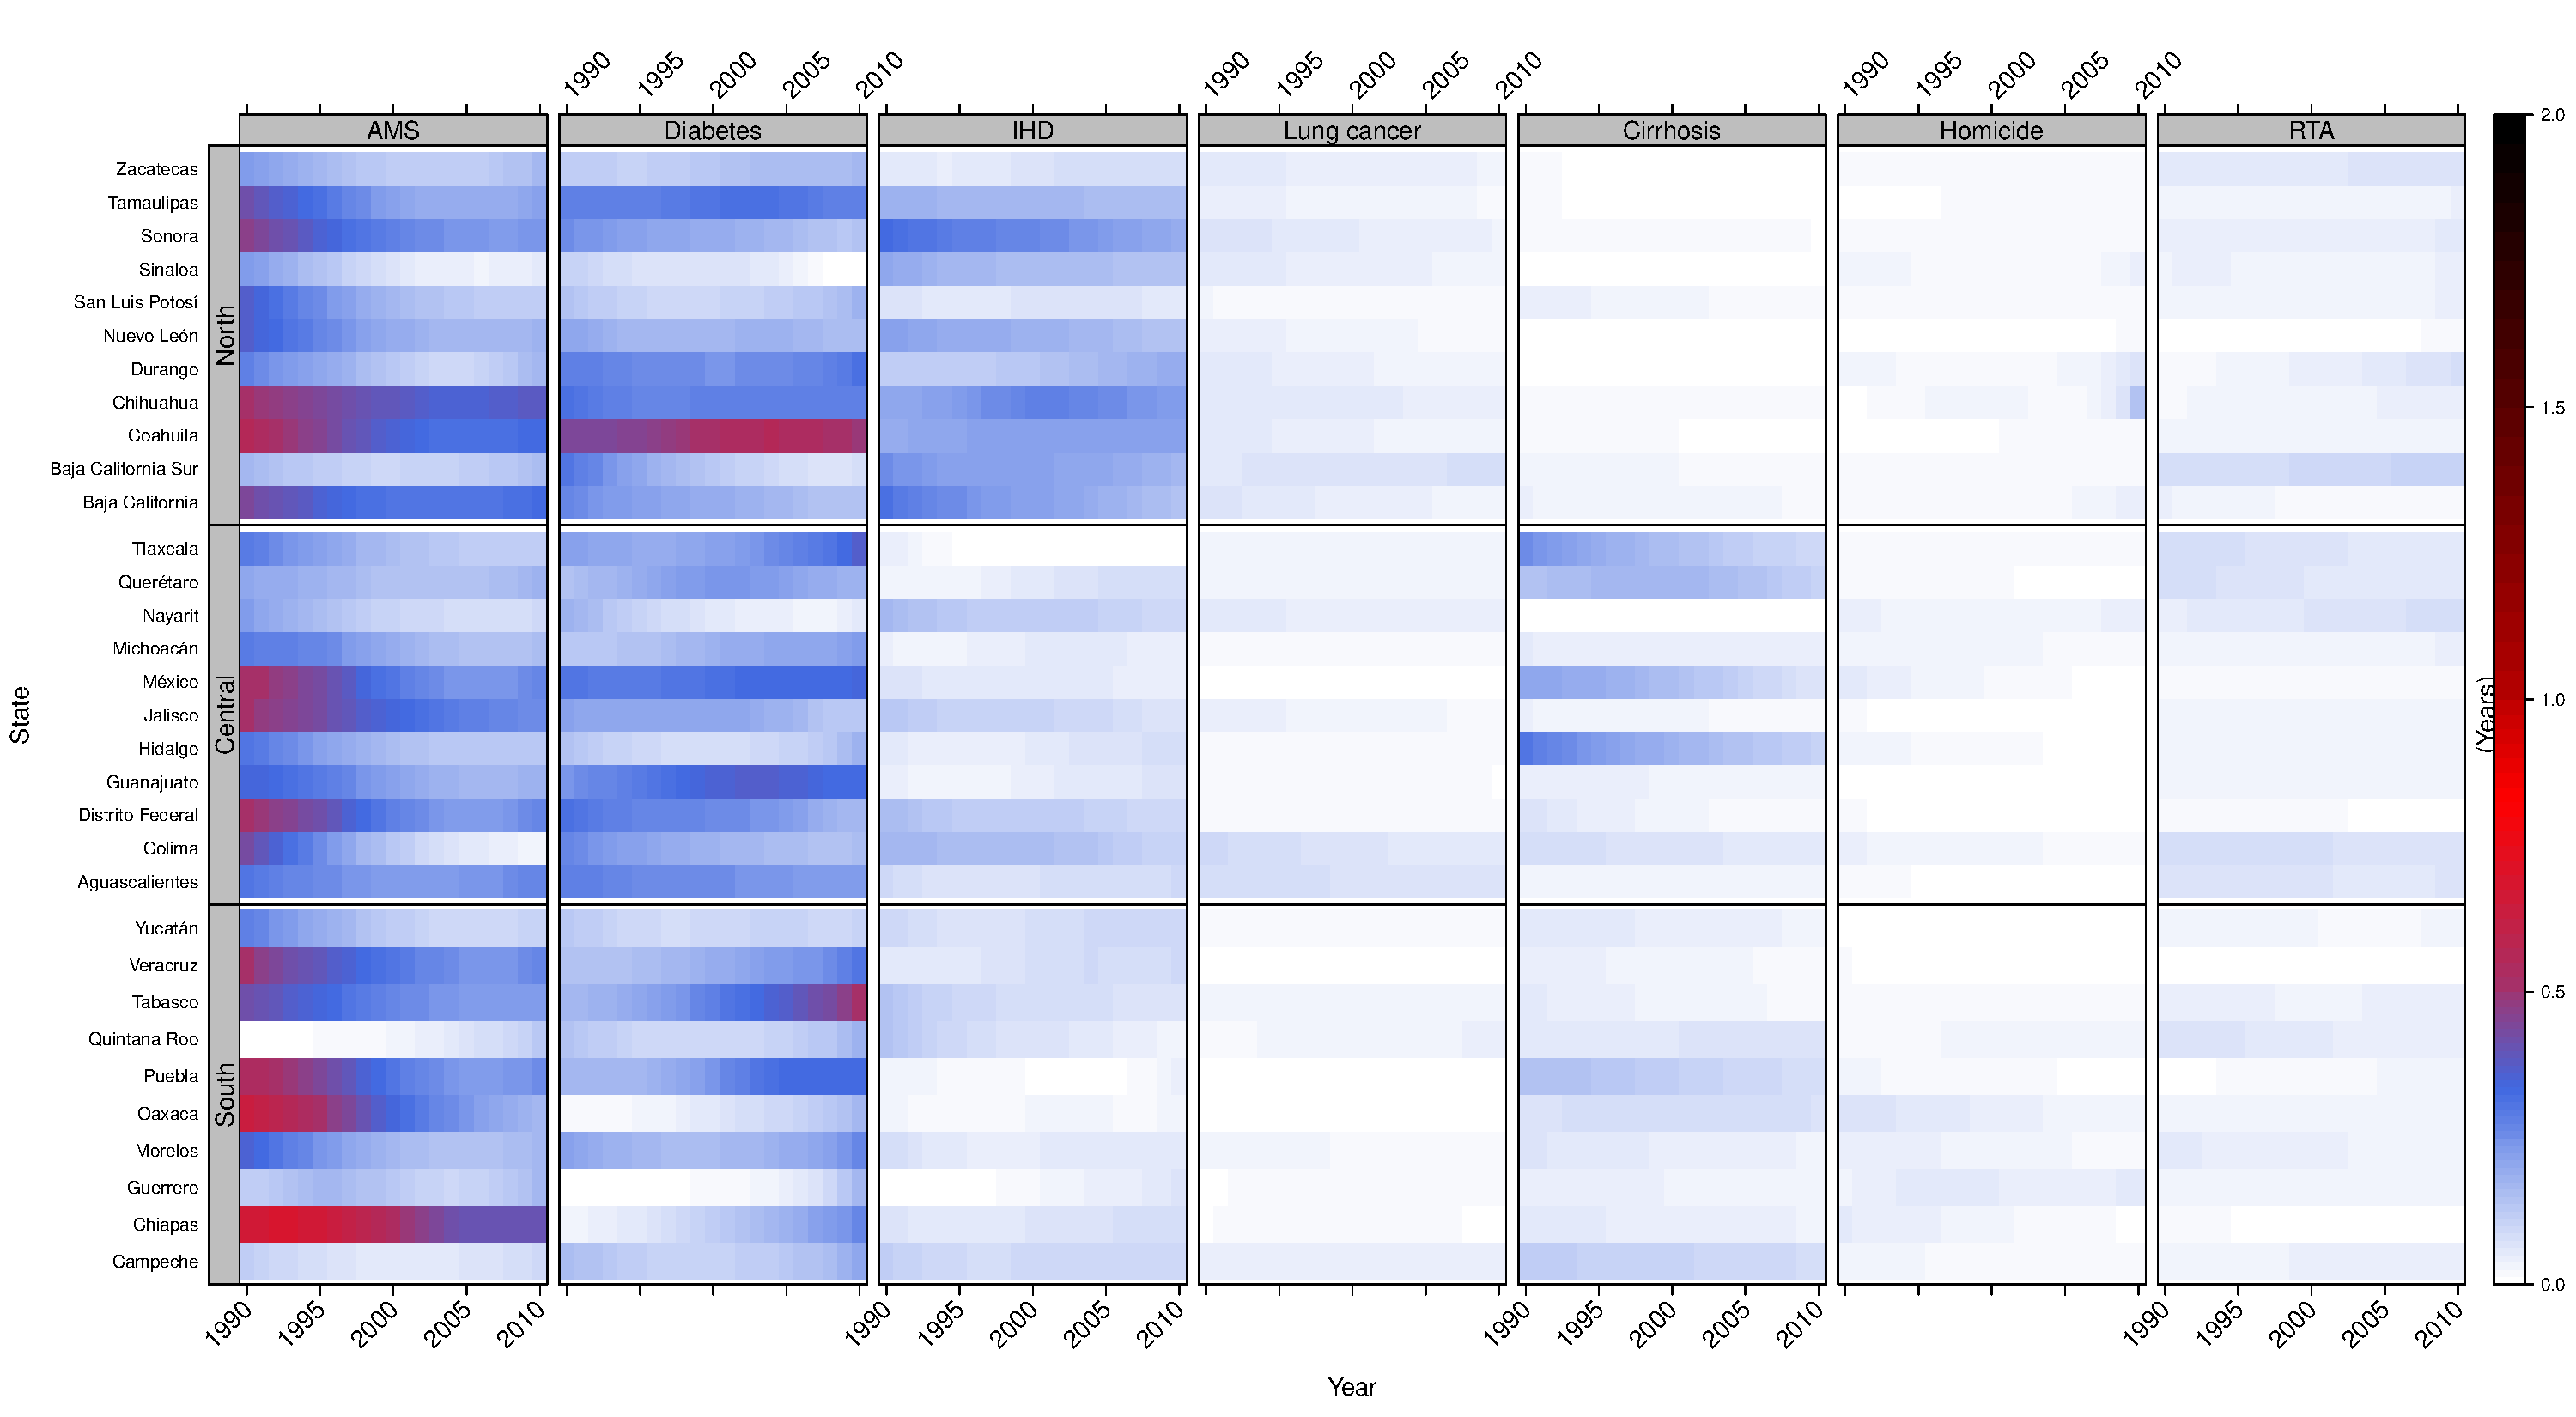
\includegraphics[scale=.33]{Figures/Adult_Female_heatmap.pdf}
Note: AMS, is the acronym for amenable to medical service, IHD for isquemic heart diseases and RTA stands for road traffic accidents. Source: own calculations based on INEGI and SOMEDE files. \end{figure}

Causes amenable to medical service follow a similar pattern for males (figure  \ref{fig:e40_74_males}). More detrimental, however, is the toll of mortality caused by diabetes and IHD. The increase in the first one has led to decreasing survival among male adults and simultaneously increasing inequalities between states, as they show very different patterns. For instance,  Tamaulipas, Coahuila (north area); Tlaxcala, M\'exico state, Guanajuato and the Federal District in the central region; along with Veracruz, Tabasco and Puebla in the south, show clear deterioration during the study period, while other states experienced improvements that led to reducing the gap towards the low mortality benchmark due to diabetes (e.g. Sinaloa in the north, Nayarit in the central region, and Yucat\'an in the south). As in females, IHD exhibit a very different pattern between regions. Almost every state from the north could gain more than one year of life if IHD mortality was reduced towards the low mortality benchmark. On the contrary, cirrhosis affects male survival mainly in the central and southern regions. Quer\'etaro, Michoac\'an, Jalisco, Puebla and Oaxaca show the largest deviations from the low mortality benchmark due to cirrhosis mortality. Finally, homicide mortality also affects older-adult survival in particular states, as the gaps between the low mortality benchmark and the observed life expectancy are wider after 2005. Similar to young adults patterns, Sinaloa, Durango, Chihuahua and Guerrero could potentially increase the survival in one year if homicide mortality converges to the low mortality benchmark. Road traffic accidents (RTA) and the rest of AM-categories do not contribute notably to the gap between the observed survival and the low mortality benchmark. 




\begin{figure}[h]
\centering
\caption{Cause-specific contributions to state differences from low mortality benchmark for older male adults, 1990-2015.}
\label{fig:e40_74_males}
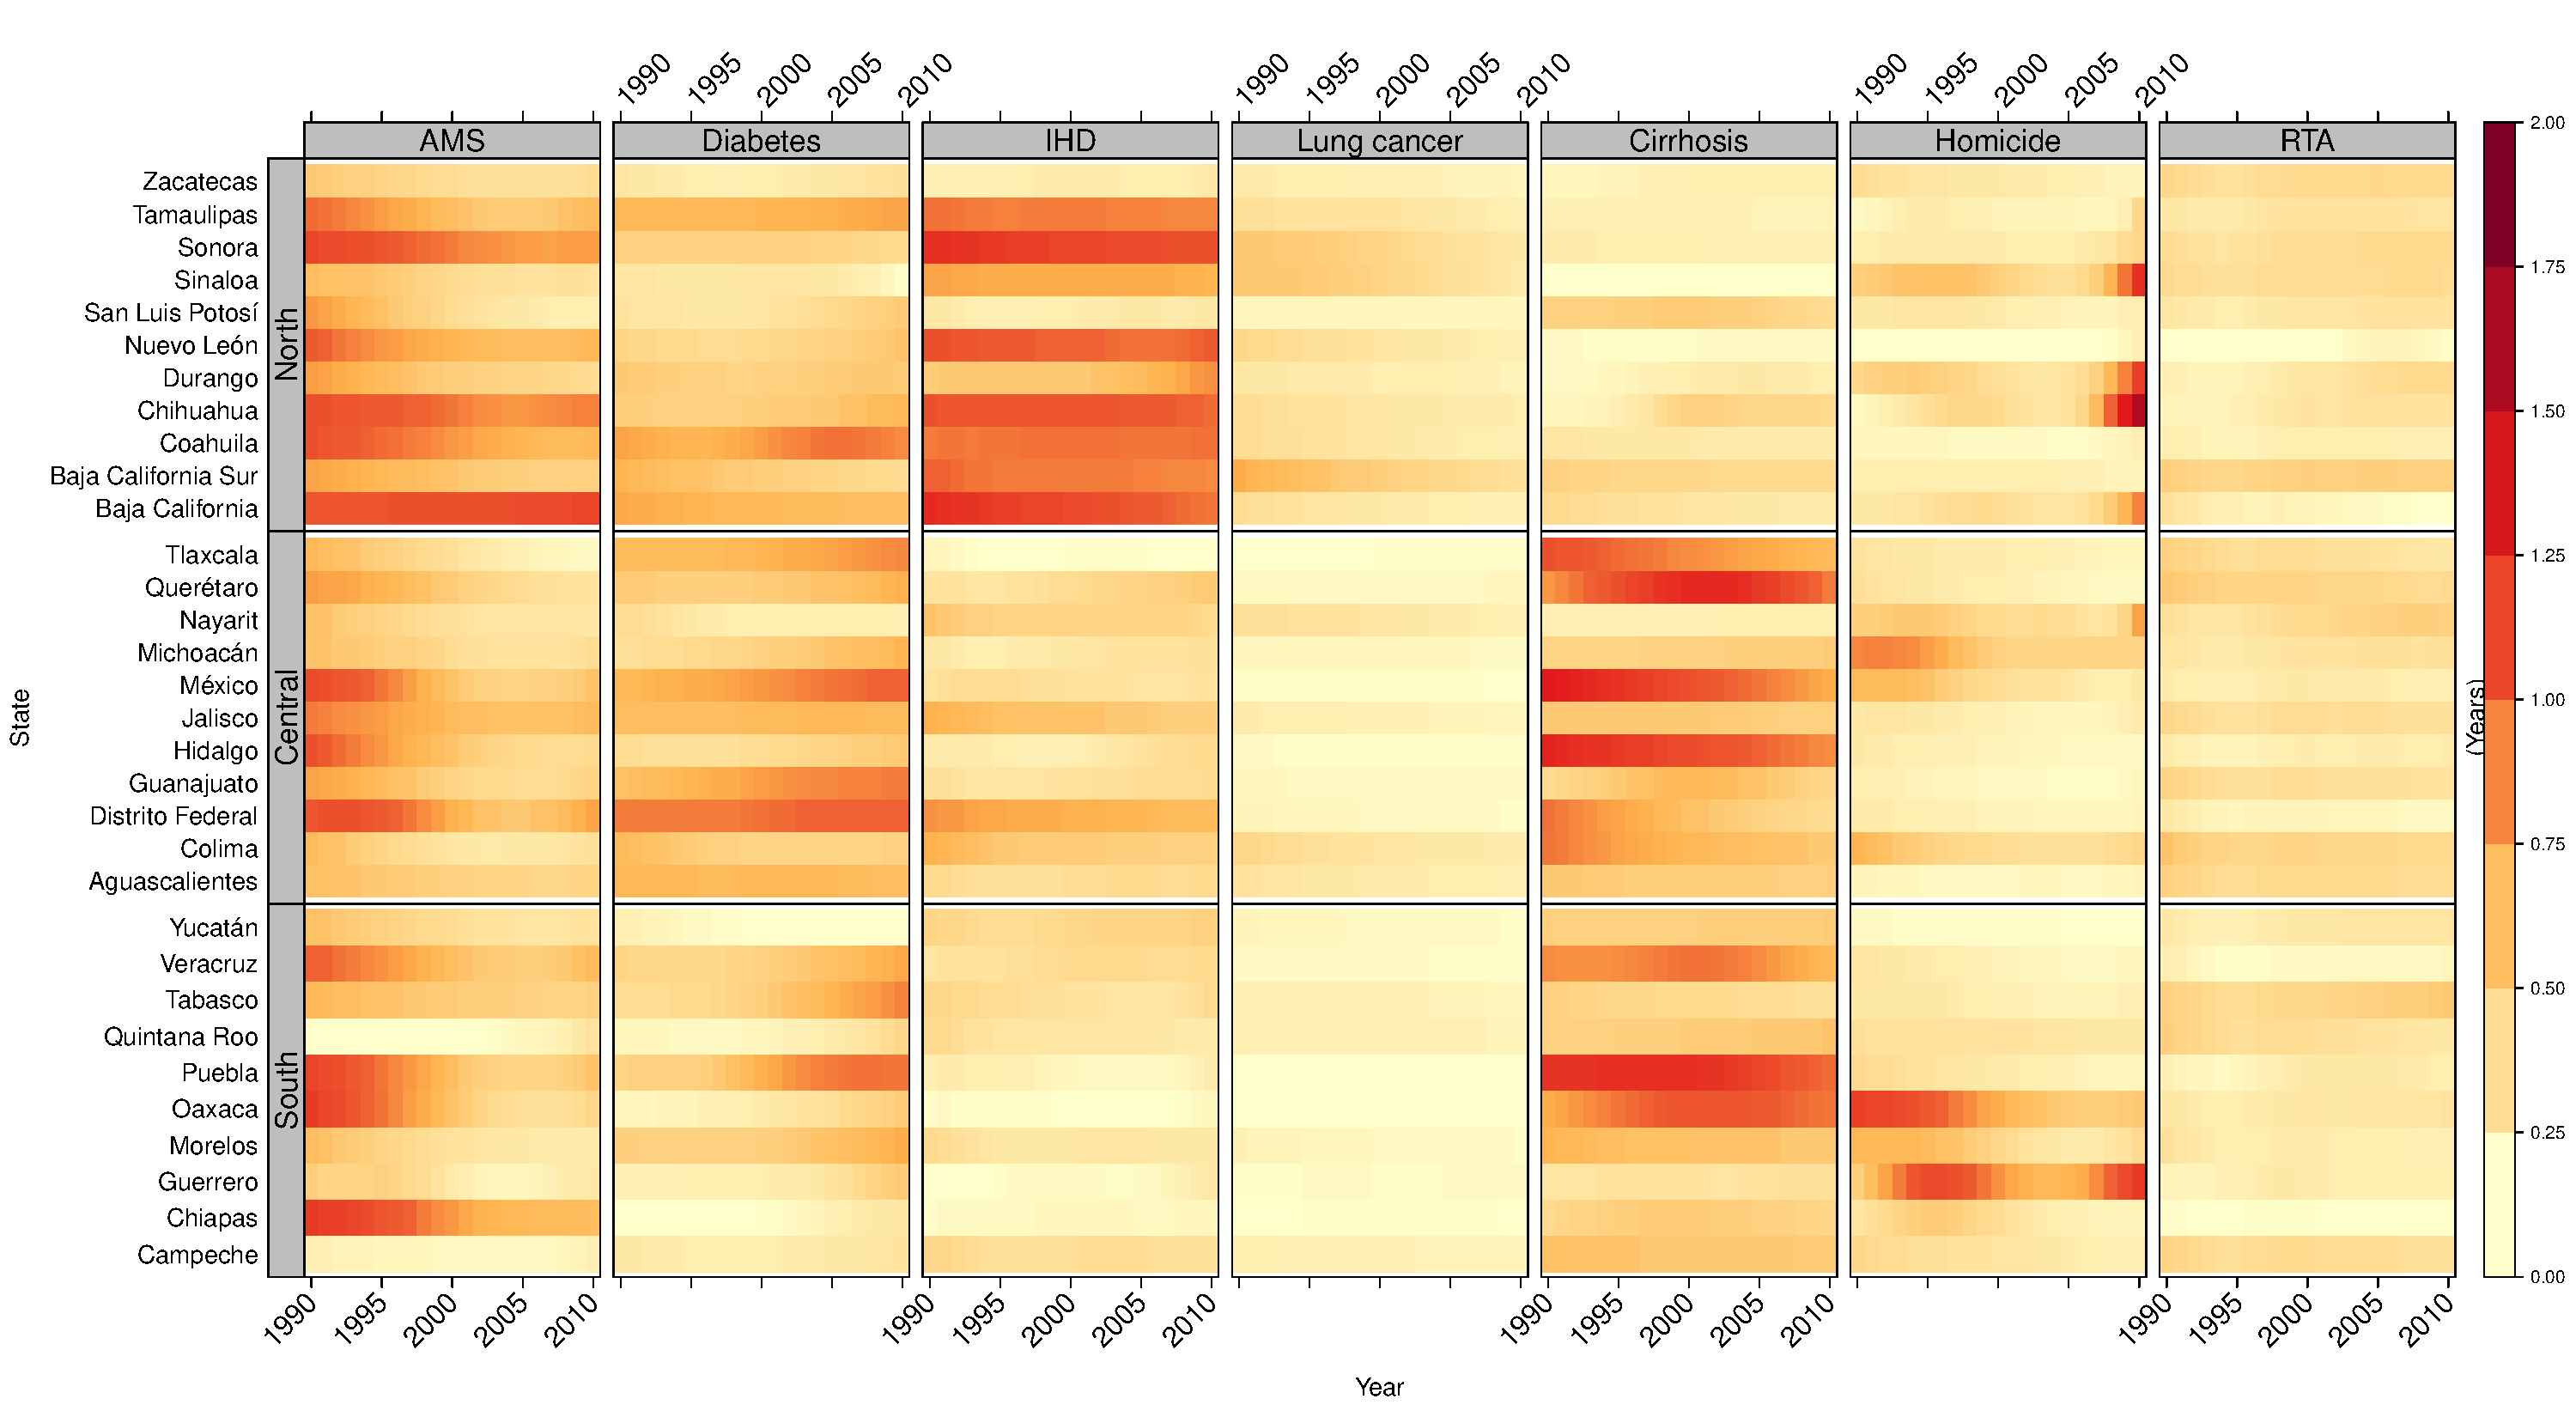
\includegraphics[scale=.33]{Figures/Adult_Male_heatmap.pdf}
Note: AMS, is the acronym for amenable to medical service, IHD for isquemic heart diseases and RTA stands for road traffic accidents. Source: own calculations based on INEGI and SOMEDE files. 
\end{figure}


All 32 states included in this analysis increased the survival between 0 and 14 years because of reductions in causes amenable to medical service in females and males (see Appendix's figures  \ref{fig:e0_14_males},\ref{fig:e15_39_males}). The transitions towards the low mortality benchmark were more intense in states in the central and southern region within males. For instance, Tlaxcala, Mexico, Puebla and Chiapas reduced the gap between the benchmark and the observed survival gaining almost one additional year of life. 

Among the young-adult population (15-39), deviations from the low mortality benchmark observed in males after 2005 were mainly driven by homicide mortality (see Appendix's figure \ref{fig:e15_39_males}). The unexpected increase of homicide led to widening the gap between the benchmark and the observed survival in almost every state. In the north region, the gap went from around a quarter of year in 2002 to more than one year by 2010 in Sinaloa (pacific coast), Durango and Chihuahua (state bordering Texas in the U.S.). Nayarit, Michoac\'an, in the central region, and Guerrero in the south were the states that showed the largest deviations due to homicide mortality following their northern counterparts. Road traffic accidents contributed to the gap between the benchmark and the observed temporary life expectancy but with a minor effect. In females, the contribution of homicide mortality after 2005 was only discernible in the state of Chihuahua (see Appendix's figure \ref{fig:e15_39_females}). Importantly, the low mortality benchmark is constructed with the minimum homicide mortality rate, these results do not imply that the rest of states did not present homicide mortality. The impact of the rest of AM categories in both, young ages and young-adults is negligible. 



%\subsection*{Age and cause contributions to state differences from the best
%practices trend.}
%This section will be completed at a later date. Preliminary results are shown.
%\begin{figure}[h!]
%\caption{Cause-specific contributions to the difference between observed and BP. (preliminar figure)}
%\centering
%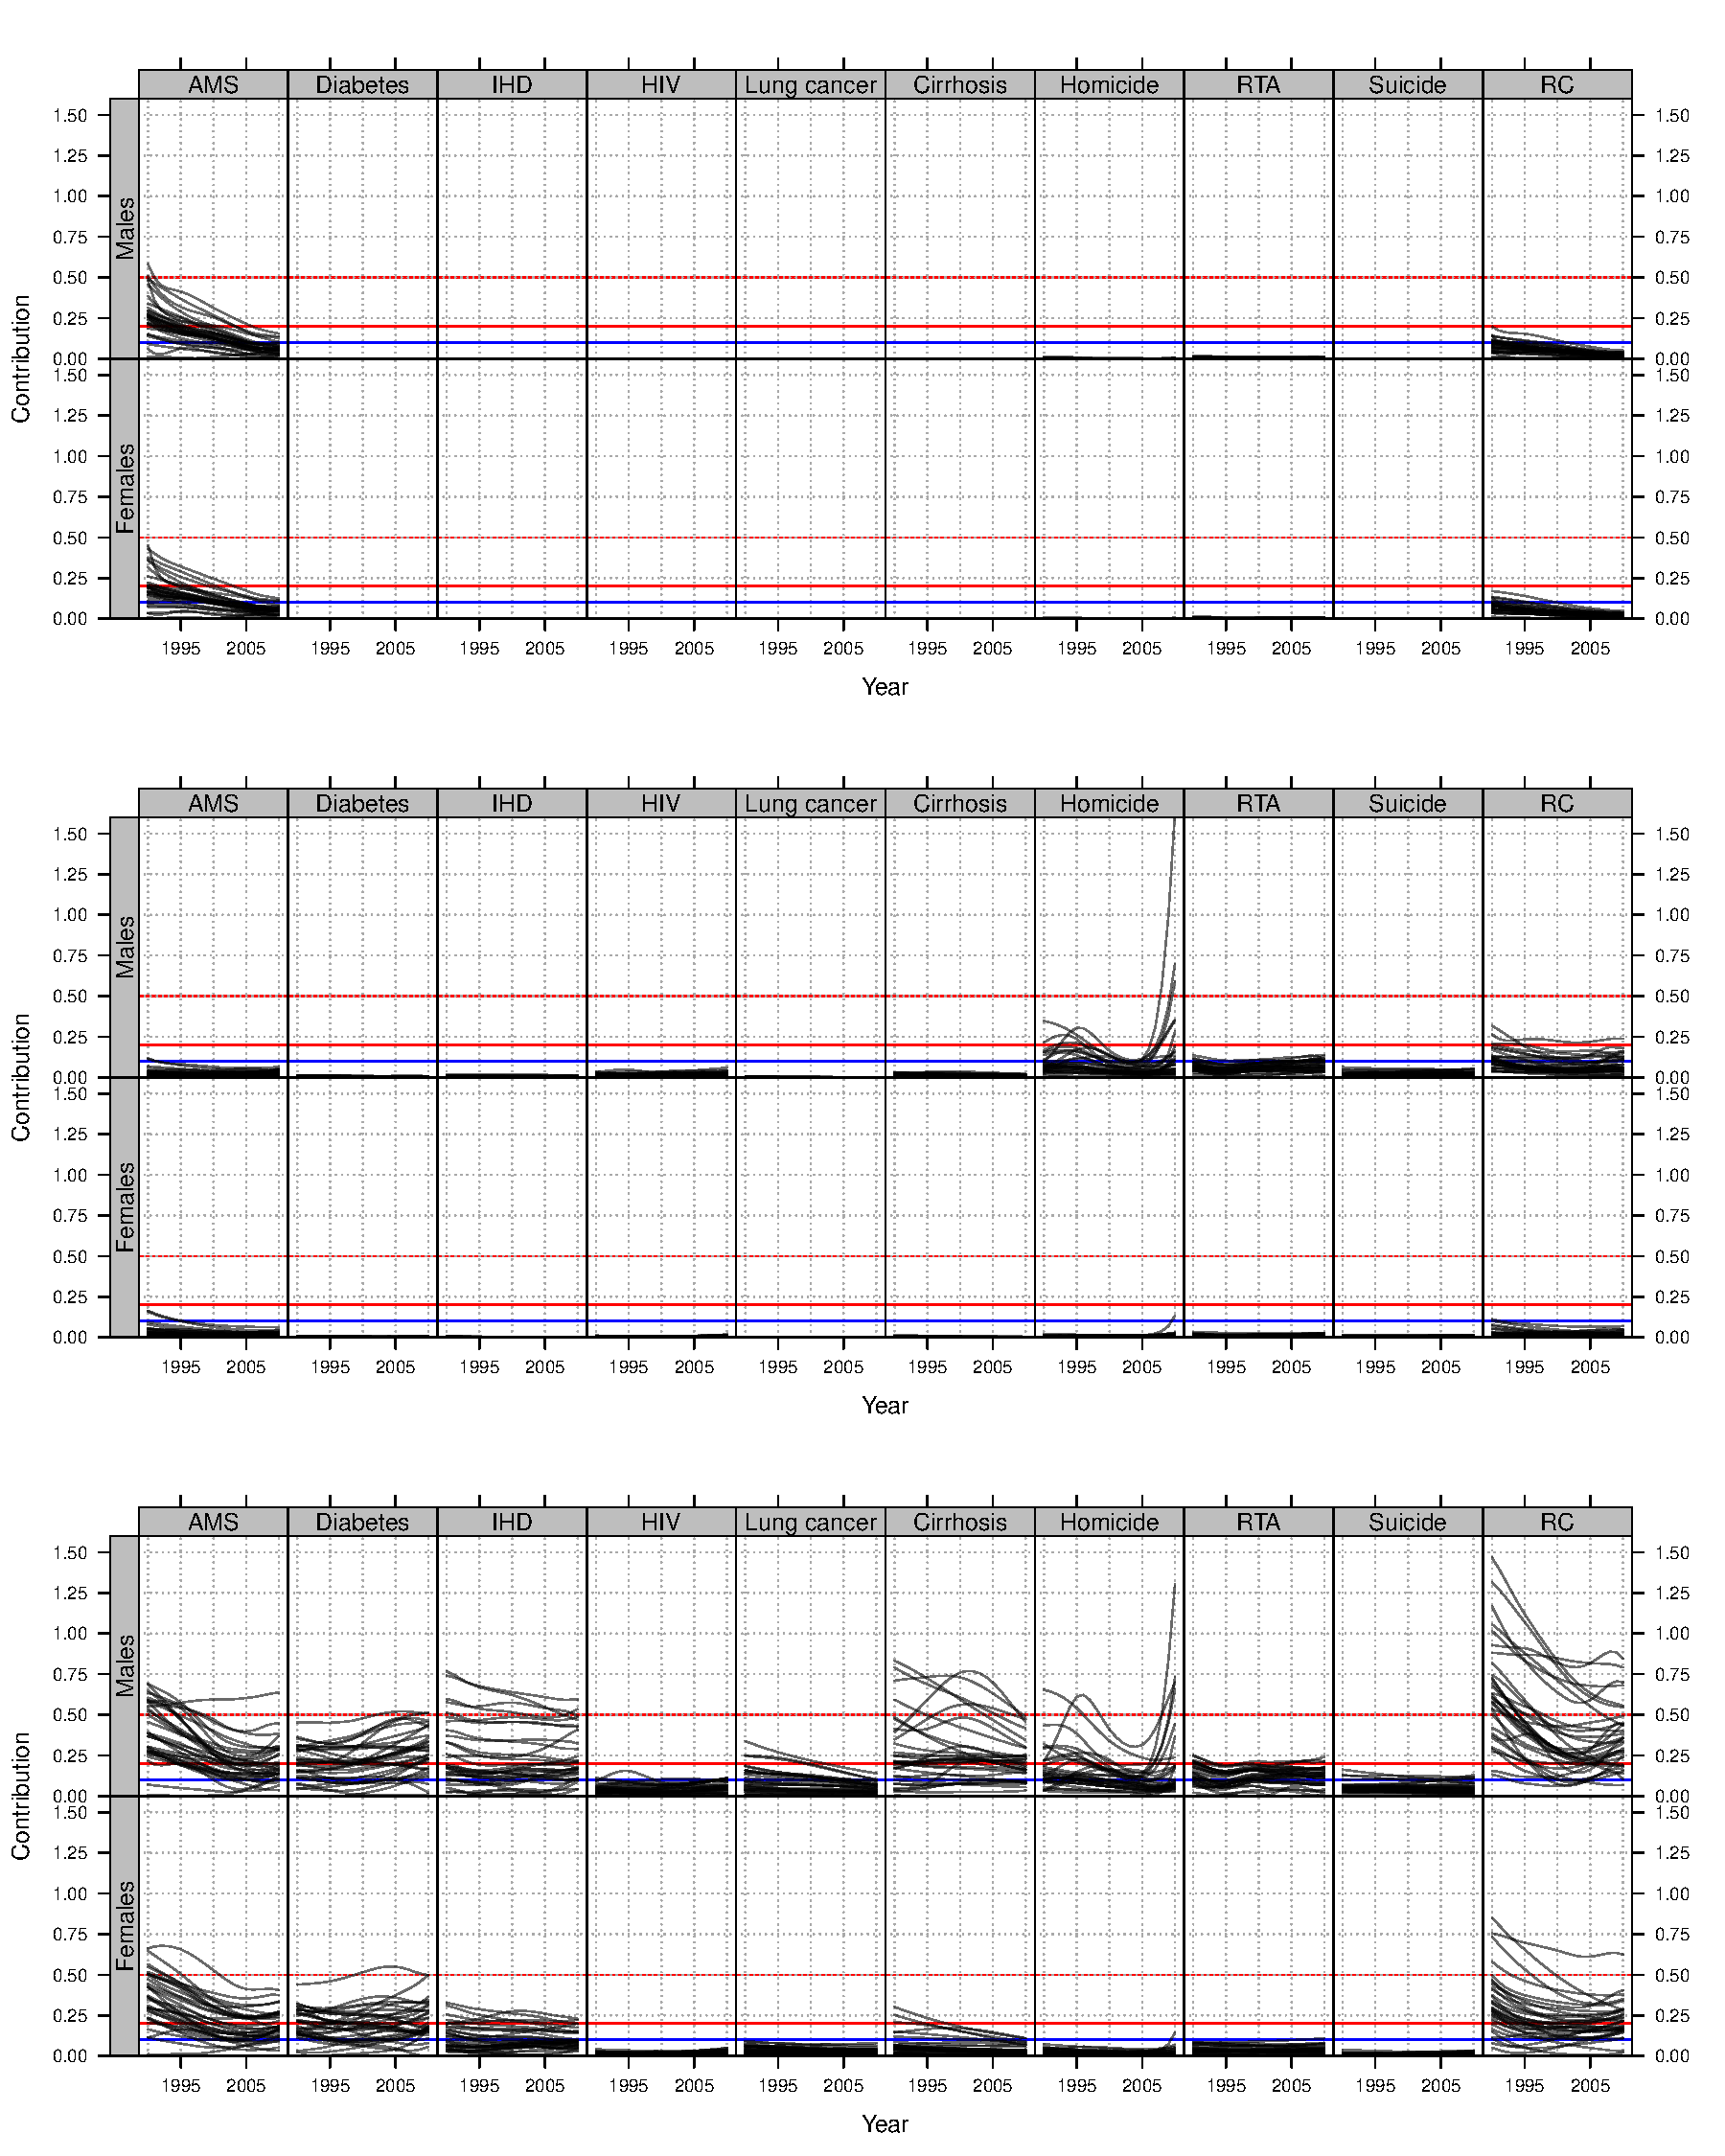
\includegraphics[scale=.4]{Figures/TLE_Decomp.pdf}
%Source: own calculations based on INEGI and SOMEDE
%\end{figure}


%This will show a few small multiples figures, tbd 

%\section*{Discussion}
%Talk about the role of homicide and other major causes. How many years of life
%were lost? (not just expectancy). maybe..

\section*{Discussion}
\subsection*{Child and young-adult mortality}
This analysis demonstrates the potential contribution of achieving the low mortality benchmark to the improvements in mortality equality and life expectancy. However, it is concerning that the low mortality benchmarks have not been steadily increasing over the period studied. Although trends were flat for children, they are experiencing almost full survival before age 15. More worrisome is the common shift after 2005 in adults and the decreasing pattern observed in older adult's low mortality benchmark. 

Despite the flattening pattern of the low mortality benchmark in children, our results show that all states in Mexico have improved survival towards this benchmark. This has been due to improvements in causes amenable to medical service, which is consistent with previous research that highlight decreases in mortality rates at younger ages due to infectious and respiratory conditions associated to public health interventions targeted to children in Mexico \citep{sepulveda2006}. For example, states like Puebla and Tlaxcala improved the survival over half a year since the 1990's, and by 2015 mortality inequality was reduced so that all states' temporary life expectancy range between 14.6 and 14.8 years. By 2012, the coverage for skilled attendance at delivery remained above 90\% and more than 78\% of children under age one visited the doctor to monitor their development and growth  \citep{urquieta2015evolution}, our results show consistency with these figures as mortality rates improved during the period. In addition, equitable vaccination coverage has been achieved for the entire young population, the success of such public health interventions are in line with our results, underscoring the improvements in survival in the population younger than 15 years associated to the progress detected in health insurance coverage due to vaccination programs and the implementation of the Seguro Popular \citep{urquieta2015evolution}. Although life expectancy in the young population has improved, there still exist areas of opportunity to achieve full-survival under age 15 in causes amenable to medical service, mainly in states in the central ans southern regions of the country. 

Young adults (population between 15 and 40 years) show a converging pattern towards the low mortality benchmark in all states just before 2005. However, an unexpected increase in homicide rates after 2005 in all states affected dramatically the male survival among the young population in the country. Previous research documented losses in the overall life expectancy up to three years in the state of Chihuahua (the bordering state with Texas, USA) and almost two years in Sinaloa, Durango (North) and Guerrero (South) between 2005 and 2010 due to homicides\citep{Aburto2015}. Our findings show that the trend towards the low mortality benchmark was reversed after 2005 due to the increase in homicide mortality, with a top in 2011. Although homicide rates decreased after 2011, they still are the main cause of death contributing to the gap between the observed survival and the low mortality benchmark in particular states (e.g. Sinaloa, Durango in the north, Nayarit and Michoac\'an in the cetral region, and Guerrero in the south). To put this in perspective, the gap between the low mortality benchmark in Chihuahua is five times higher than the gap in the beginning of the 1990's. 
These results underscore the need of effective interventions to reduce homicide mortality, as it still contributes the most to survival deterioration among the young-adult population and mortality inequality among states. Even ten years after the national security strategy that aimed at reducing drug cartels' operations started and homicides begun to spread all over the country\citep{espinal2015analysis}, the toll of homicide on life expectancy deterioration is appalling. Between-state variance in temporary life expectancy was much smaller for females over the same period, though females showed the same overall trend of convergence, followed by divergence after 2005.

\subsection*{Older-adult mortality}
In Mexico, since the beginning of the 1990's, survival at adult ages (40-75) deteriorated for males and stayed steady for females. Our research sheds some light on this pattern by showing that the low mortality benchmark decreased as a result of offsetting state-mortality trends and the interaction between improvements in causes amenable to medical service (e.g. infectious and respiratory diseases) and deterioration in diabetes and isquemic heart diseases, and in behavior-related mortality (e.g. cirrhosis, homicides). 

Out of 35 potential years, adult females in Mexico are living less than 33 and males less than 31 since the 1990's. The increase in  diabetes, isquemic heart diseases and cirrhosis mortality is at the heart of survival's deterioration, with clear regional variations. Although improvements in causes amenable to medical service were witnessed, almost every state still has chance to improve, in particular the northern states of Sonora, Chihuahua and Baja California. In spite of this progress, diabetes mortality increased over the period and contributed to widening the gap to achieve the low mortality benchmark. Diabetes-related mortality increased 23\% from 1998 to 2002 and the prevalence of diabetes was estimated at 14.4\% in the adult population in 2006, these figures underscore the emerging epidemic of diabetes, which is larger in Mexico compared with other Latin American countries \citep{glassman2010confronting}. To put this in perspective, Coahuila, the state of Mexico, Guanajuato, the Federal District, Tabasco and Puebla could increase the survival in almost one year if diabetes mortality were to achieve the low mortality benchmark. Similarly, mortality related to isquemic heart diseases (IHD) contributes to lowering life expectancy in adults. We identified a clear regional pattern in the country, almost all the states in the Northern region could potentially benefit with one additional year in life expectancy if the low mortality benchmark were reached, where as the central and southern regions present a lower effect of IHD. Opposing this, cirrhosis-related mortality shows a higher impact in the southern and central states of the country, particularly in Quer\'etaro, M\'exico state, Hidalgo (central area) and Puebla and Oaxaca in the south. Both diabetes and IHD mortality are closely related to obesity prevalence, previous research anticipated that the increasing levels of obesity in Mexico could compromise gains in life expectancy \citep{monteverde2010obesity}, our findings suggest that the toll of these causes of death on population's health is such that adults are not surviving as much as they potentially could. In this regard, a recent taxation exercise to reduce the consumption of sugar sweetened beverages showed positive results in the short term after its implementation to reduce purchases \citep{colchero2016beverage}. However, the long term implications are unknown, but if they remain health outcomes should improve and lessen the burden of obesity-related mortality.

There is still room for improvements to reduce state-mortality differences and improve the survival among the adult population in Mexico. Several screening and prevention strategies (e.g. PREVENIMSS) for early diabetes and hypertension have been implemented in the country. However, as previous research have found, they are far from achieving the ultimate goal and including the entire population \citep{castro2010potential}. In addition, a recent study shows that the conditional cash transfer program PROGRESA/Oportunidades improves health significantly for adult women \citep{behrman2013health}. Nevertheless, the results are not the same for men since the program is not oriented to males, nor the adult population itself. 




\subsection*{Conclusion}
Improving health is a priority for governments of many developing countries, in part to achieve the Millennium Development Goals established for 2015.  Great improvements have been accomplished in reducing mortality and inequalities in children and the young population. Nevertheless, our results show that older adults are becoming a vulnerable group and more efforts are require to reduce the burden of conditions amenable to health services and policy/related conditions. In particular, this group lacks efforts on attending the burden of violence, through homicides; chronic-degenerative
causes of death, such as diabetes and isquemic heart diseases; and behavior-related conditions like cirrhosis.  

There is no simple way to lessen the impact of such conditions, but it is clear that new approaches are needed to improve survival in the adulthood and to minimize health disparities between states, as they still remain. Preventing diabetes, isquemic heart diseases and obesity requires fundamental social and political challenges \citep{hossain2007obesity}. Therefore,  public health initiatives should focus in health care for chronic conditions as recently suggested by \citet{knaul2015achieving}, but they should also influence the population towards improving health behavior. Our results reinforce the need of such, among others public health interventions, with an special focus on older adults in the Mexico. 


\end{spacing}

\section*{Competing interest}
None to declare.

%However, they still remain the world's most unequal countries \citep{Barreto2012}.
%}
%\bibliographystyle{plainnat}
\newpage
 \bibliography{AburtoRiffe_Bib.bib}
 
 
 \newpage
\section*{Supplemental material}
Appendix Table 1. Definitions of cause-of-death categories using the \nth{9} and \nth{10} revision of the International Classification of Diseases.\\

{\renewcommand{\baselinestretch}{1}\selectfont

\begin{longtable}{p{8cm}p{4cm}p{4cm}ccc}
\hline
\textbf{Category} & \textbf{ICD-10} & \textbf{ICD-9}\\
\hline
\endfirsthead
\multicolumn{3}{c}%
{\tablename\ \thetable\ -- \textit{Continue}} \\
\hline
\textbf{Category} & \textbf{ICD-10} & \textbf{ICD-9}\\
\hline
\endhead
\hline \multicolumn{3}{r}{\textit{Continues}} \\
\endfoot
\hline
\endlastfoot
\multicolumn{3}{l}{\bf I. Amenable to medical service}  \\
 I.A. AM-Infectious \& respiratory diseases : intestinal infections, tuberculosis, zoonotic bacterial diseases, other bacterial diseases, septicemia, poliomyelitis, measles, rubella, infectious hepatitis, ornithosis, rickettsioses/ arthropod-borne, syphilis (all forms), yaws, respiratory diseases, influenza \& pneumonia, chronic lower respiratory diseases & A00-A09, A16-A19, B90, A20-A26, A28, A32, A33, A35, A36, A37, A40-A41, A80, B05-B06, B15-B19, A70, A68, A75, A77, A50-A64, A66, J00-J08, J20-J39, J60-J99, J09-J18, J40-J47 & 001-009, 010-018, 32, 33, 37, 137, 020-027, 38, 45, 55-56, 70, 73, 080-082, 087, 090-099, 102, 460-479, 500-519, 480-488, 490-496 \\
           I.B. AM-Cancers: malignant neoplasm of colon, skin, breast, cervix, prostate, testis, bladder, kidney-Wilm's tumor only, eye, thyroid carcinoma, Hodgkin’s disease, leukemia & C16,C18-C21, C43-C44, C50, C53, C61, C62, C67, C64, C69, C73, C81, C91-C95 & 153-154, 172-173, 174, 180, 185, 186, 188-189, 190, 193, 201, 204-208\\
           I.C. AM-Circulatory: active/acute rheumatic fever, chronic rheumatic heart disease, hypertensive disease, cerebrovascular disease & I00-I02, I05-I09, I10-I13, I15, I60-I69 & 390-392, 393-398, 401-405, 430-438\\
          I.D. AM-Birth: maternal deaths (all), congenital cardiovascular anomalies, perinatal deaths (excluding stillbirths) & O00-O99, Q20-Q28, P00-P96 & 630-676, 745-747, 760-779\\
          I.E. AM-Other: disease of thyroid, epilepsy, peptic ulcer, appendicitis, abdominal hernia, cholelithiasis \& cholecystitis, nephritis, benign prostatic hyperplasia, misadventures to patients during surgical or medical care, cisticerchosis & E00-E07, 40-G41, K25-K27, K35-K38, K40-K46, K80-K81,  N00-N07, N17-N19, N25-N27, N40, Y60-Y69, Y83-Y84, B69 & 240-246, 345, 531-533, 540-543, 550-553, 574-575.1, 580-589, 600, E870-E876, E878-E879\\
 & \\          
 {\bf II. Diabetes}  & E10-E14 & 250 \\      
 & \\
 {\bf III. Ischemic Heart Diseases (IHD)}   & I20-I25 & 410-414, 429.2\\
 & \\           
 {\bf IV. HIV/AIDS} & B20-B24 & 279.1, 042-044\\ 
  & \\                
{\bf V. Lung cancer}  & C33-C34 & 162\\
  & \\          
{\bf VI. Cirrhosis}&  K70 & 571.1-571.3\\
 & \\          
{\bf VII. Homicides}  & X85-Y09 & E960-E969\\     
 & \\           
 {\bf VIII. Road traffic accidents}  & V01-V99 & E810-E819 \\     
 & \\           
{\bf IX. Suicide and self-inflicted injuries}  & U03, X60-X84, Y87.0 & E950-E959\\ 
 & \\          
{\bf X. Residual Causes }:  other cancers and other heart diseases & C00-D48, I00-I99 if not listed above, R00-R99 & 140-239, 390-459 if not listed above, 780-799
\label{ME_Mex}
\end{longtable}


\begin{figure}
\centering
\caption{Cause-specific contributions to state differences from low mortality benchmark for male young people, 1990-2015.}
\label{fig:e0_14_males}
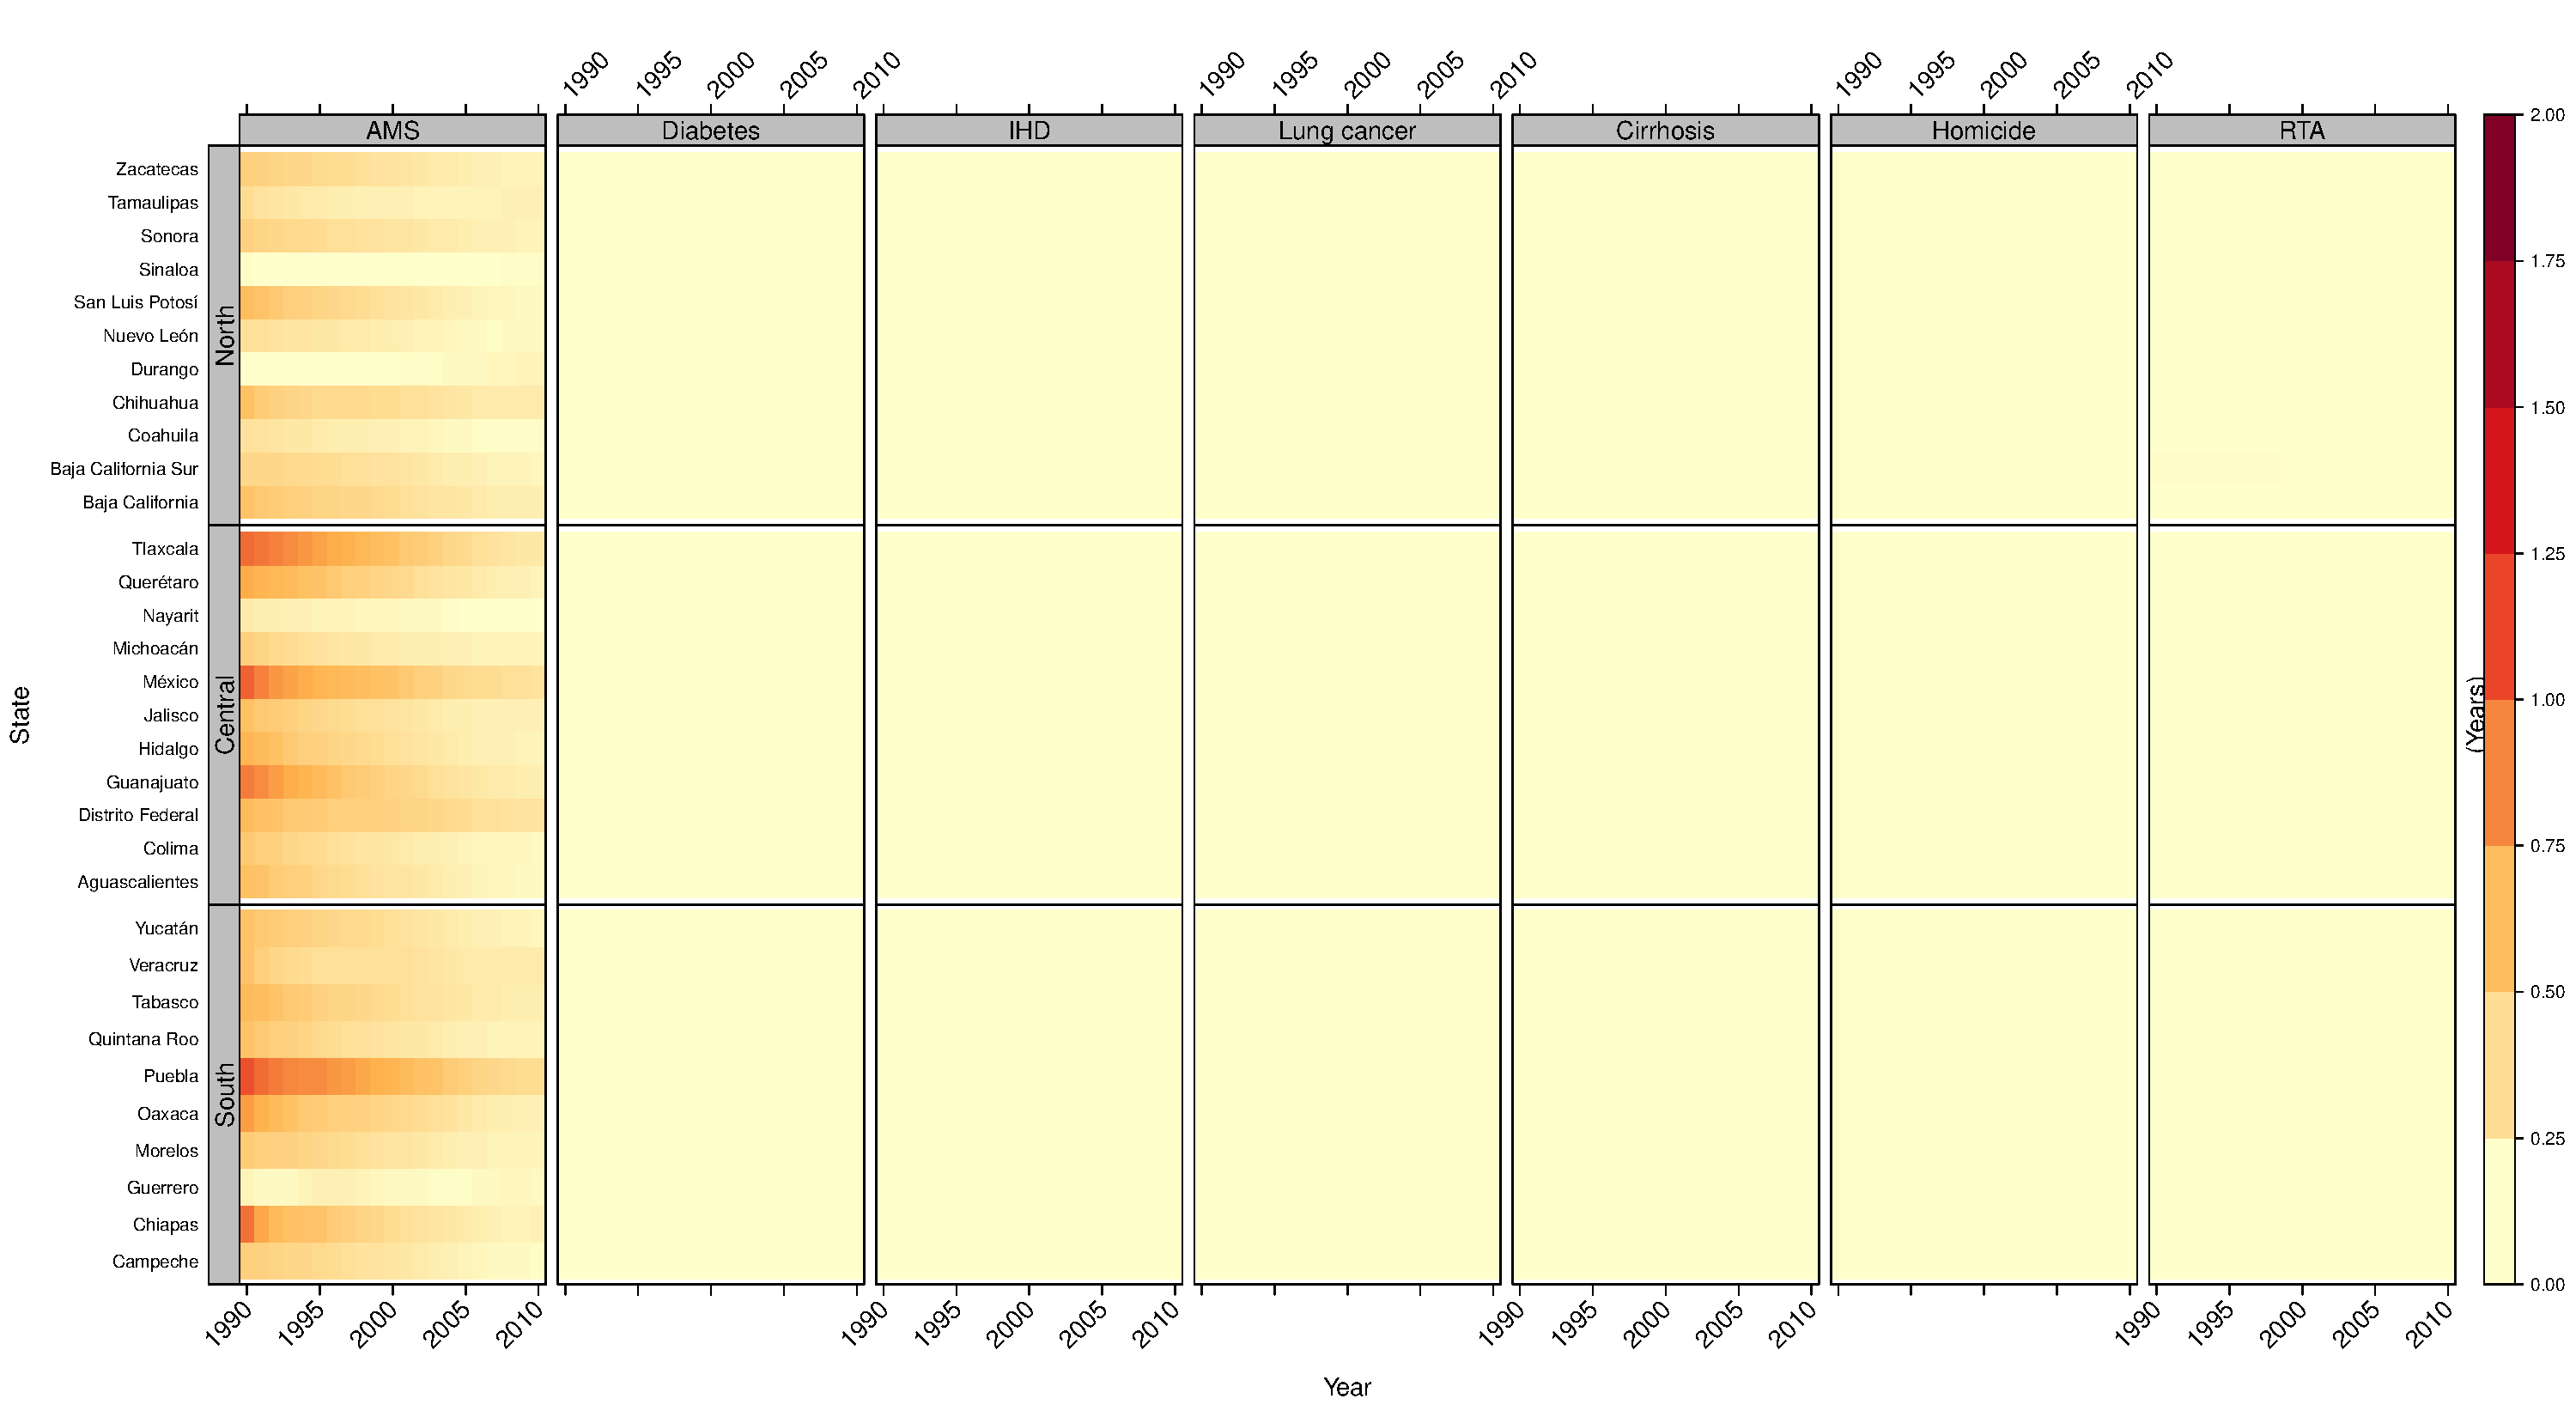
\includegraphics[scale=.3]{Figures/Young_Male_heatmap.pdf}
Note: AMS, is the acronym for amenable to medical service, IHD for isquemic heart diseases and RTA stands for road traffic accidents. Source: own calculations based on INEGI and SOMEDE files. \end{figure}

\begin{figure}
\centering
\caption{Cause-specific contributions to state differences from low mortality benchmark for female young people, 1990-2015.}
\label{fig:e0_14_females}
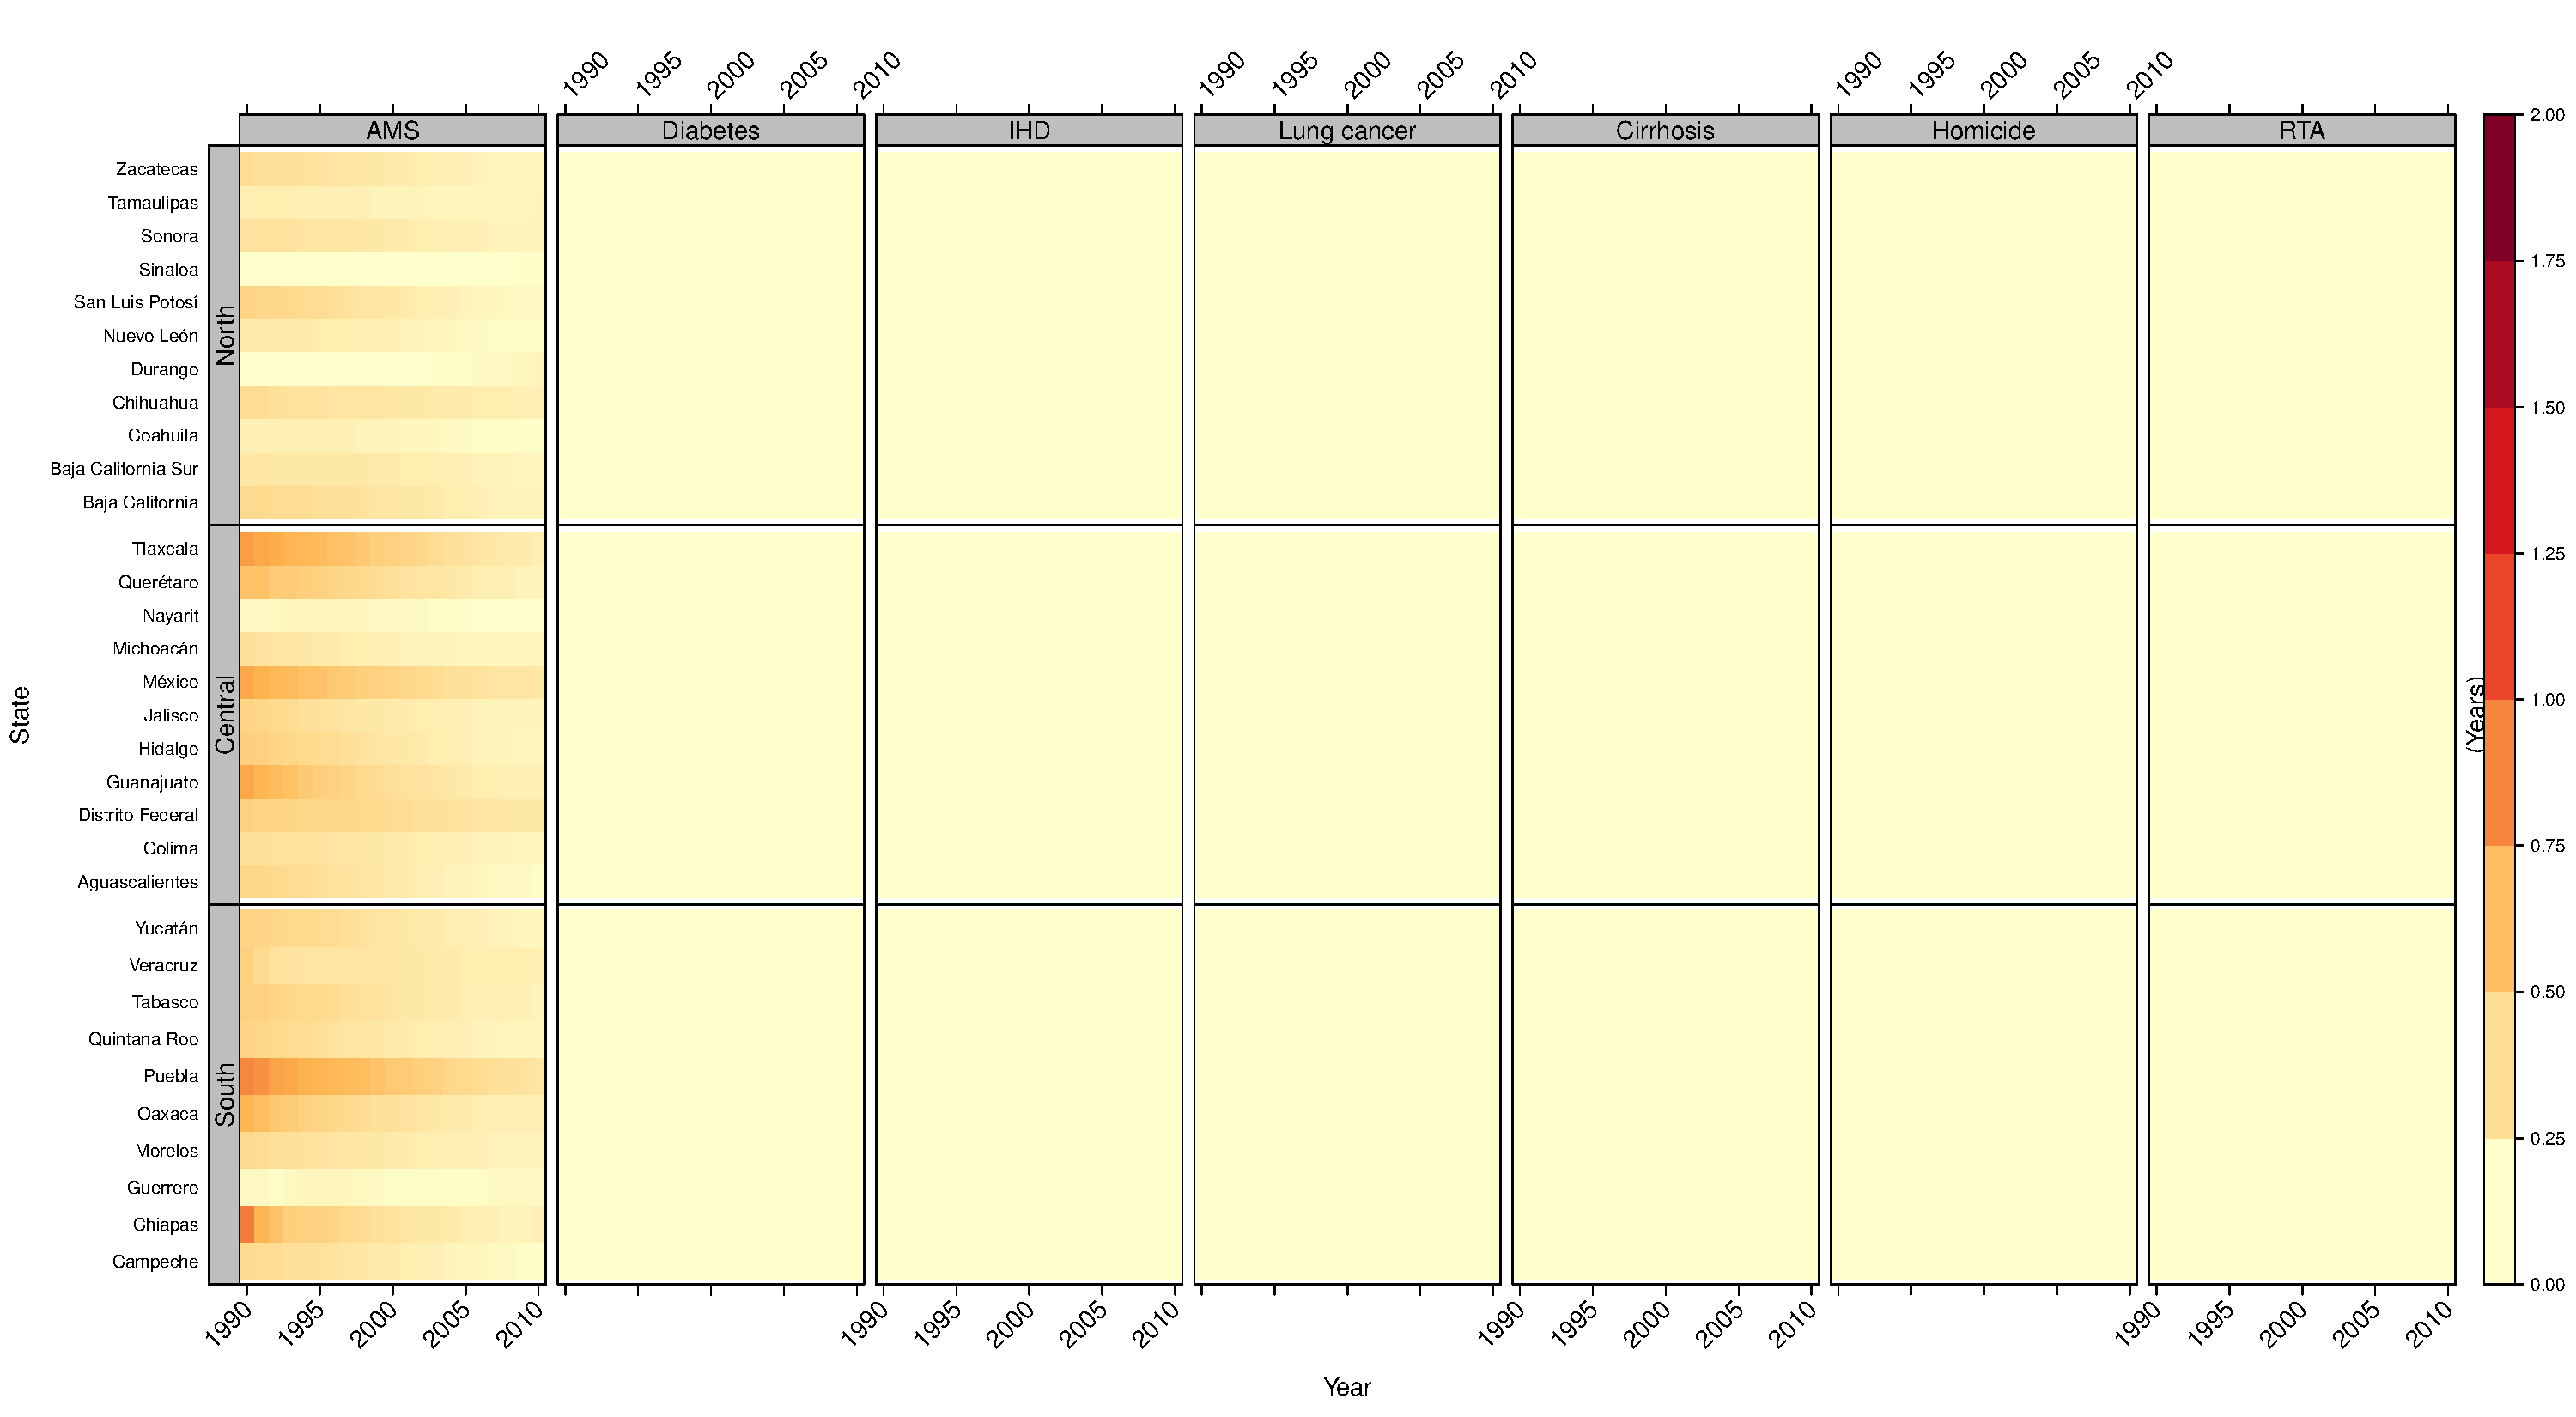
\includegraphics[scale=.3]{Figures/Young_Female_heatmap.pdf}
Note: AMS, is the acronym for amenable to medical service, IHD for isquemic heart diseases and RTA stands for road traffic accidents. Source: own calculations based on INEGI and SOMEDE files. \end{figure}



\begin{figure}
\centering
\caption{Cause-specific contributions to state differences from low mortality benchmark for male young adults, 1990-2015.}
\label{fig:e15_39_males}
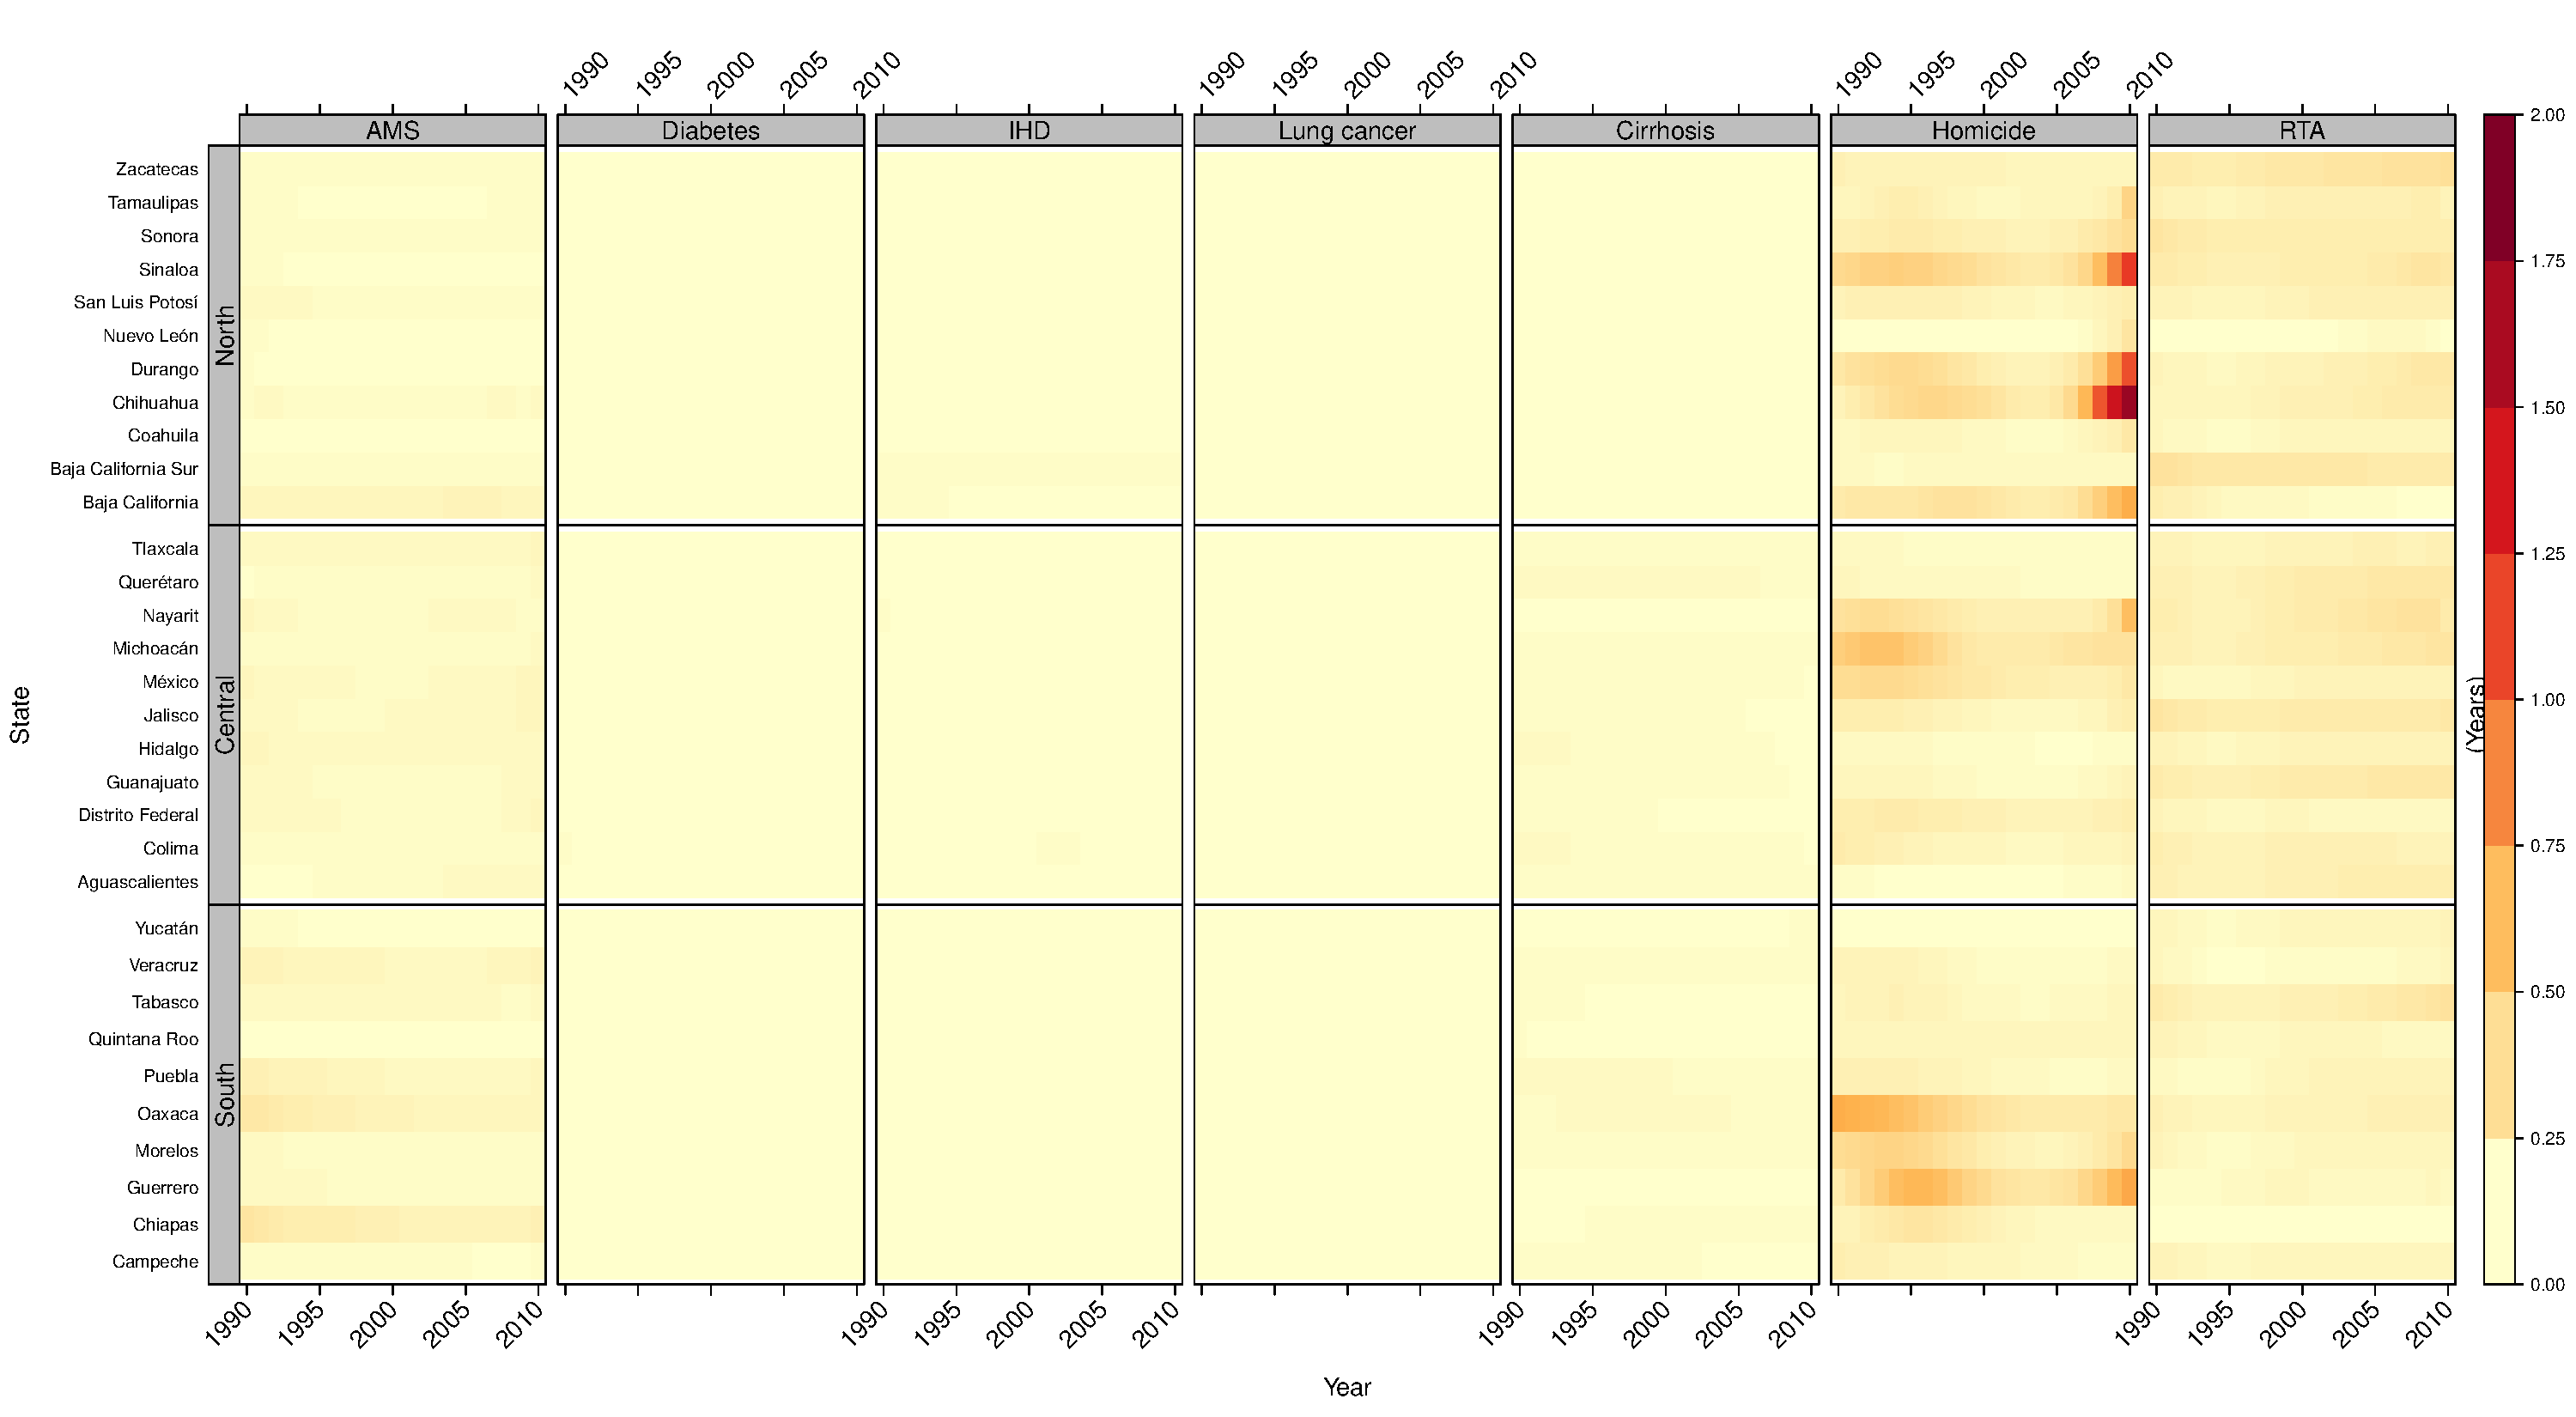
\includegraphics[scale=.3]{Figures/YoungAdult_Male_heatmap.pdf}
Note: AMS, is the acronym for amenable to medical service, IHD for isquemic heart diseases and RTA stands for road traffic accidents. Source: own calculations based on INEGI and SOMEDE files. 
\end{figure}

\begin{figure}
\centering
\caption{Cause-specific contributions to state differences from low mortality benchmark for female young adults, 1990-2015.}
\label{fig:e15_39_females}
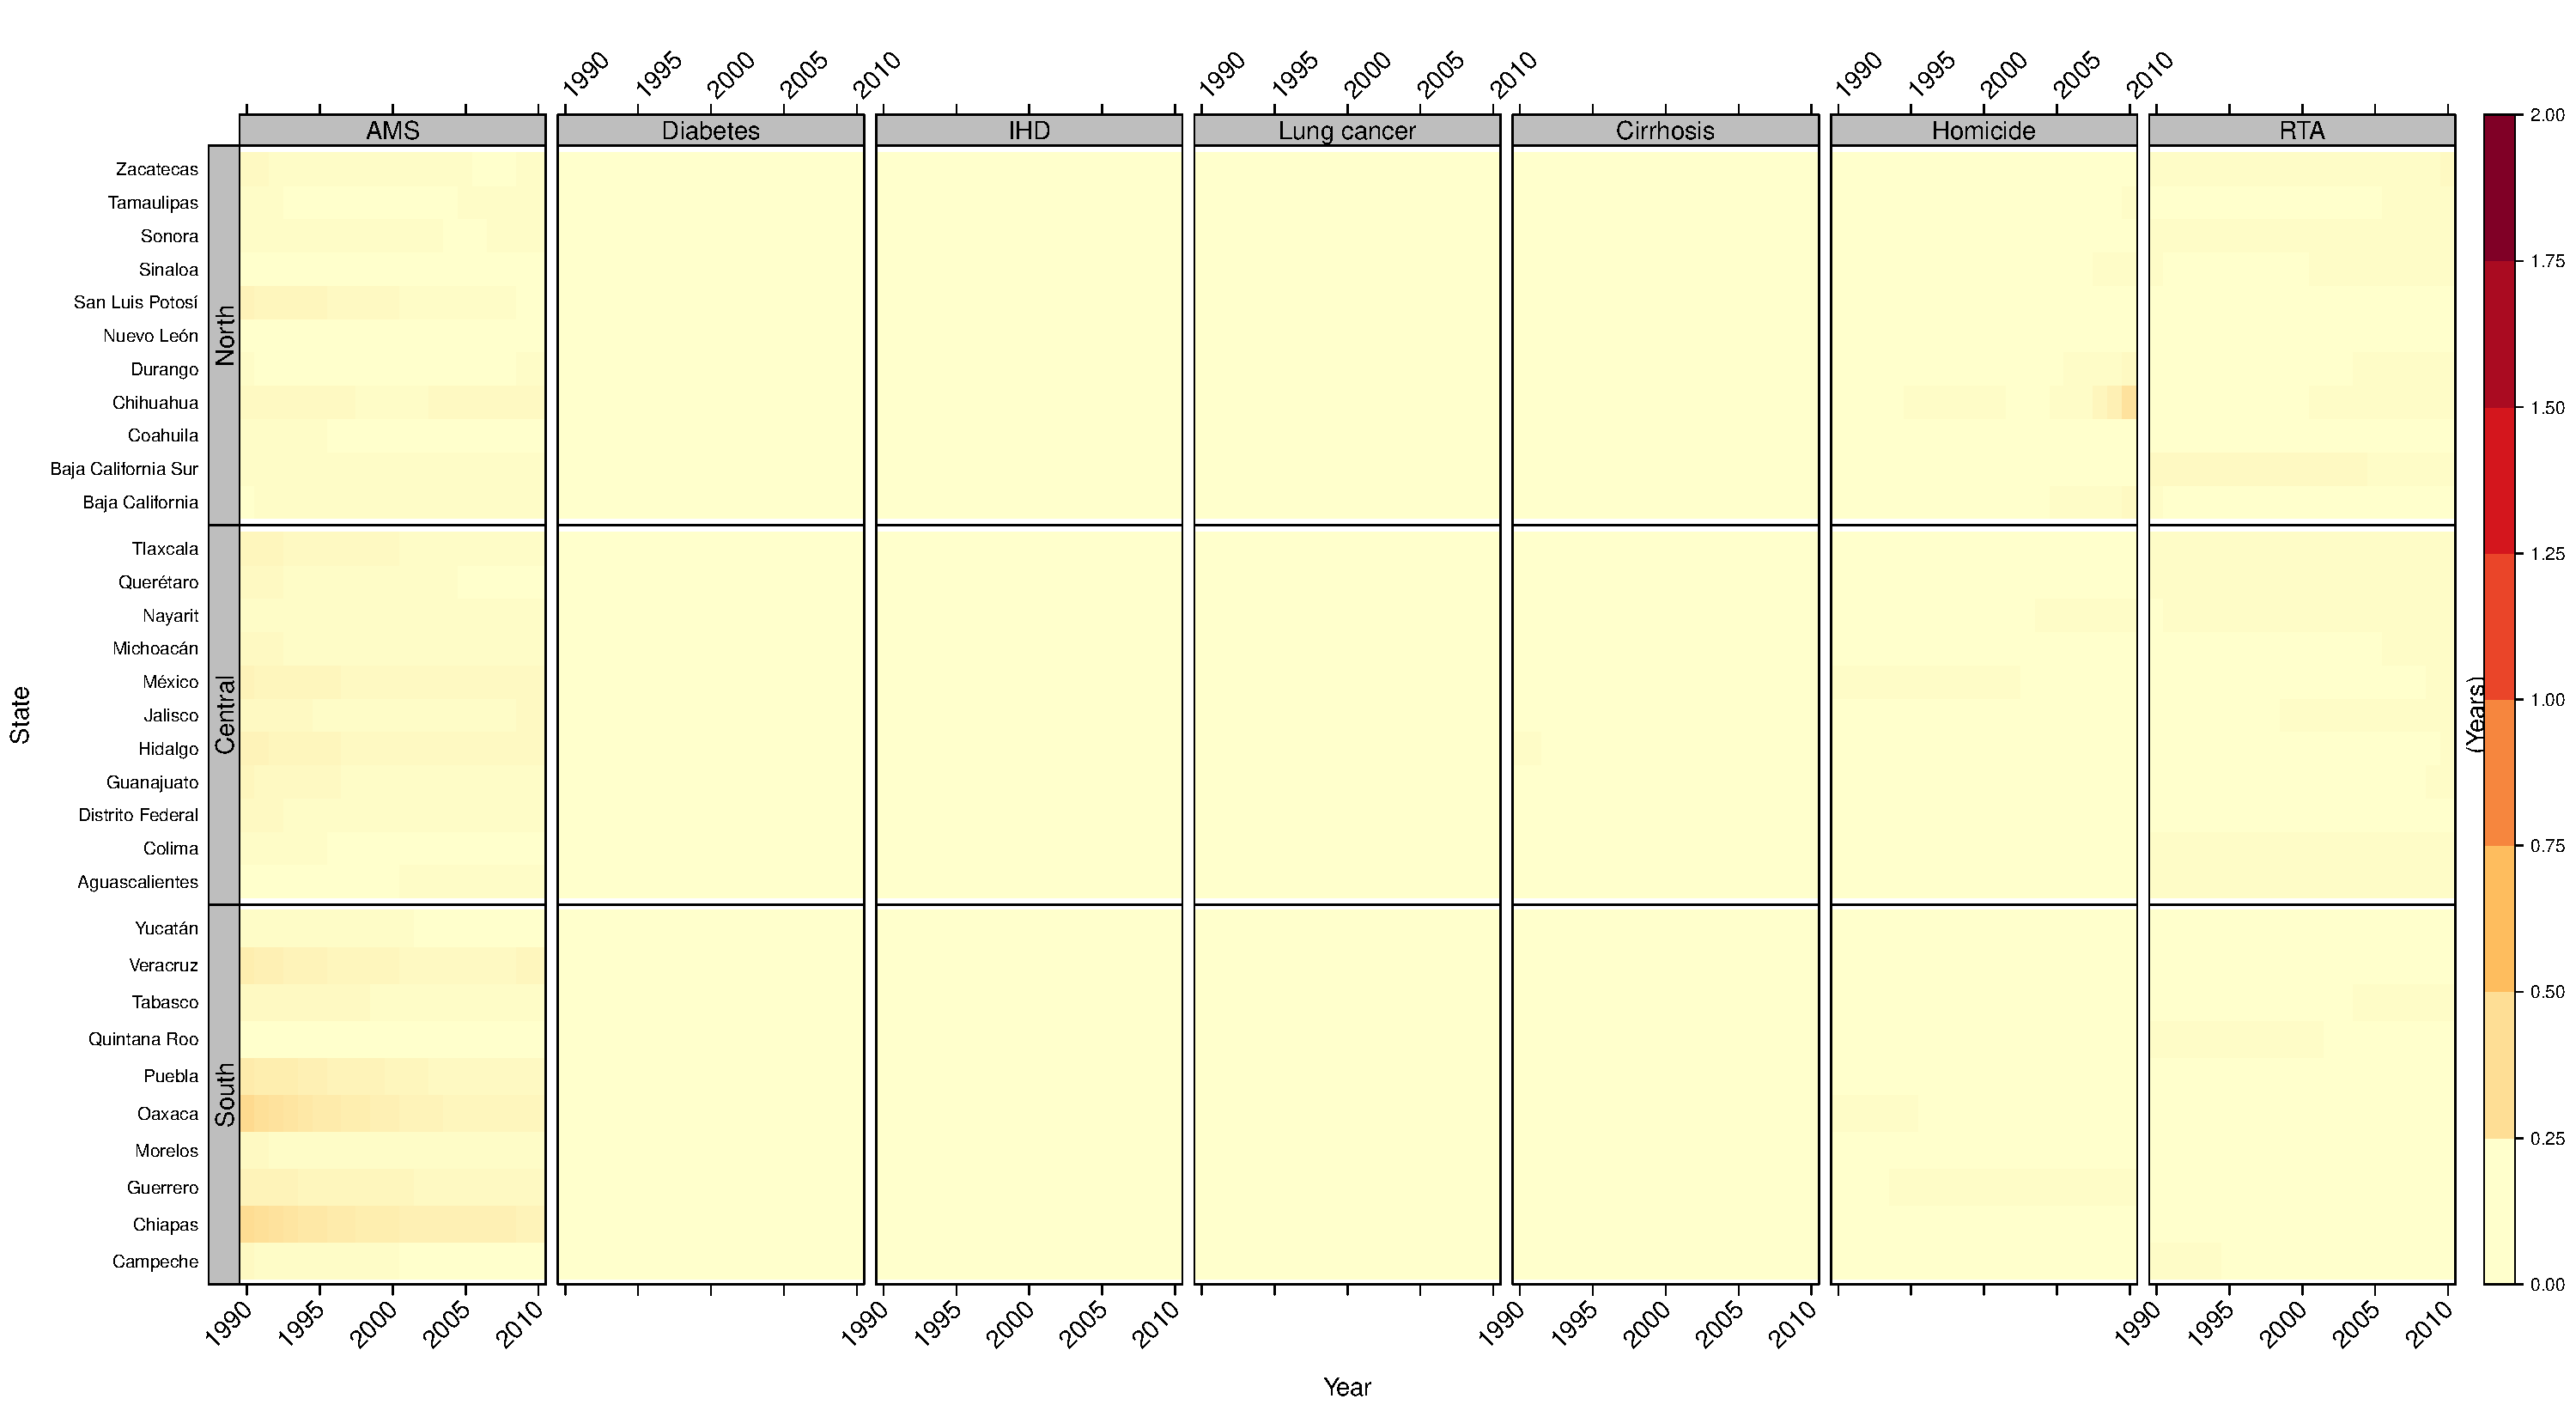
\includegraphics[scale=.3]{Figures/YoungAdult_Female_heatmap.pdf}
Note: AMS, is the acronym for amenable to medical service, IHD for isquemic heart diseases and RTA stands for road traffic accidents. Source: own calculations based on INEGI and SOMEDE files. 
\end{figure}



\begin{landscape}

% latex table generated in R 3.2.2 by xtable 1.8-0 package
% Wed Feb  3 15:51:09 2016
\begin{table}[ht]
\caption{Selected cause-specific contributions to deviations from low mortality benchmark, male older-adults by state and years, 2000, 2005 and 201}
\rowcolors{1}{}{lightgray}
\begin{footnotesize}
\centering
\begin{tabular}{lllll|lll|lll|lll|lll|lll}
\hline
Region & State &  \multicolumn{3}{c}{Amenable to M.S} & \multicolumn{3}{c}{Diabetes} &  \multicolumn{3}{c}{IHD} &  \multicolumn{3}{c}{Lung cancer}&  \multicolumn{3}{c}{Cirrhosis}&  \multicolumn{3}{c}{Homicide}\\
  \hline
& Year  & 2000 & 2005 & 2010 & 2000 & 2005 & 2010 & 2000 & 2005 & 2010 & 2000 & 2005 & 2010 & 2000 & 2005 & 2010 & 2000 & 2005 & 2010 \\ 
  \hline
  
North & Baja California & 0.59 & 0.6 & 0.64 & 0.3 & 0.29 & 0.28 & 0.62 & 0.55 & 0.47 & 0.1 & 0.08 & 0.06 & 0.12 & 0.1 & 0.09 & 0.16 & 0.12 & 0.44 \\ 
   & Baja California Sur & 0.26 & 0.22 & 0.21 & 0.22 & 0.19 & 0.16 & 0.46 & 0.45 & 0.42 & 0.22 & 0.18 & 0.14 & 0.18 & 0.17 & 0.16 & 0.08 & 0.07 & 0.06 \\ 
   & Coahuila & 0.4 & 0.32 & 0.3 & 0.38 & 0.48 & 0.42 & 0.49 & 0.47 & 0.49 & 0.11 & 0.09 & 0.07 & 0.1 & 0.09 & 0.09 & 0.03 & 0.02 & 0.08 \\ 
   & Chihuahua & 0.47 & 0.4 & 0.45 & 0.22 & 0.25 & 0.3 & 0.57 & 0.54 & 0.49 & 0.12 & 0.1 & 0.09 & 0.2 & 0.18 & 0.17 & 0.17 & 0.13 & 1.3 \\ 
   & Durango & 0.22 & 0.2 & 0.16 & 0.2 & 0.23 & 0.23 & 0.24 & 0.3 & 0.41 & 0.09 & 0.08 & 0.06 & 0.09 & 0.1 & 0.08 & 0.14 & 0.13 & 0.65 \\ 
   & Nuevo Le\'on & 0.32 & 0.28 & 0.31 & 0.17 & 0.2 & 0.26 & 0.52 & 0.48 & 0.53 & 0.12 & 0.09 & 0.07 & 0.02 & 0.03 & 0.03 & 0 & 0 & 0.09 \\ 
   & San Luis Potos\'i & 0.16 & 0.1 & 0.08 & 0.12 & 0.17 & 0.23 & 0.09 & 0.1 & 0.11 & 0.04 & 0.04 & 0.04 & 0.23 & 0.21 & 0.16 & 0.1 & 0.06 & 0.09 \\ 
   & Sinaloa & 0.17 & 0.14 & 0.14 & 0.12 & 0.1 & 0.02 & 0.34 & 0.35 & 0.32 & 0.2 & 0.15 & 0.1 & 0 & 0 & 0 & 0.22 & 0.14 & 0.73 \\ 
   & Sonora & 0.46 & 0.39 & 0.39 & 0.21 & 0.19 & 0.17 & 0.64 & 0.61 & 0.59 & 0.19 & 0.14 & 0.1 & 0.08 & 0.07 & 0.08 & 0.09 & 0.09 & 0.18 \\ 
   & Tamaulipas & 0.28 & 0.23 & 0.29 & 0.31 & 0.33 & 0.37 & 0.46 & 0.44 & 0.43 & 0.13 & 0.1 & 0.07 & 0.07 & 0.06 & 0.05 & 0.06 & 0.06 & 0.18 \\ 
   & Zacatecas & 0.16 & 0.14 & 0.16 & 0.08 & 0.11 & 0.15 & 0.09 & 0.08 & 0.1 & 0.07 & 0.06 & 0.05 & 0.08 & 0.08 & 0.08 & 0.1 & 0.08 & 0.06 \\ 
  Central & Aguascalientes & 0.21 & 0.19 & 0.2 & 0.3 & 0.3 & 0.28 & 0.15 & 0.17 & 0.17 & 0.1 & 0.08 & 0.07 & 0.22 & 0.21 & 0.21 & 0.04 & 0.04 & 0.06 \\ 
   & Colima & 0.12 & 0.1 & 0.14 & 0.19 & 0.19 & 0.21 & 0.23 & 0.22 & 0.21 & 0.12 & 0.11 & 0.09 & 0.31 & 0.27 & 0.24 & 0.16 & 0.14 & 0.18 \\ 
   & Distrito Federal & 0.34 & 0.24 & 0.37 & 0.48 & 0.52 & 0.51 & 0.34 & 0.31 & 0.29 & 0.04 & 0.03 & 0.02 & 0.27 & 0.21 & 0.16 & 0.06 & 0.04 & 0.06 \\ 
   & Guanajuato & 0.2 & 0.16 & 0.19 & 0.38 & 0.44 & 0.46 & 0.13 & 0.15 & 0.16 & 0.03 & 0.03 & 0.03 & 0.31 & 0.26 & 0.19 & 0.03 & 0.02 & 0.04 \\ 
   & Hidalgo & 0.25 & 0.17 & 0.17 & 0.16 & 0.2 & 0.25 & 0.07 & 0.13 & 0.17 & 0.02 & 0.02 & 0.01 & 0.61 & 0.51 & 0.42 & 0.06 & 0.03 & 0.03 \\ 
   & Jalisco & 0.3 & 0.27 & 0.29 & 0.29 & 0.3 & 0.3 & 0.25 & 0.24 & 0.22 & 0.07 & 0.06 & 0.04 & 0.24 & 0.22 & 0.2 & 0.07 & 0.04 & 0.09 \\ 
   & M\'exico & 0.25 & 0.2 & 0.25 & 0.39 & 0.47 & 0.51 & 0.14 & 0.12 & 0.13 & 0.01 & 0.01 & 0.01 & 0.59 & 0.47 & 0.34 & 0.15 & 0.11 & 0.1 \\ 
   & Michoac\'an & 0.16 & 0.13 & 0.15 & 0.2 & 0.26 & 0.32 & 0.11 & 0.13 & 0.15 & 0.05 & 0.04 & 0.03 & 0.21 & 0.22 & 0.23 & 0.2 & 0.2 & 0.19 \\ 
   & Nayarit & 0.14 & 0.11 & 0.1 & 0.08 & 0.08 & 0.07 & 0.19 & 0.19 & 0.17 & 0.12 & 0.09 & 0.06 & 0.07 & 0.08 & 0.08 & 0.16 & 0.15 & 0.37 \\ 
   & Quer\'etaro & 0.23 & 0.16 & 0.14 & 0.23 & 0.26 & 0.33 & 0.16 & 0.2 & 0.24 & 0.04 & 0.04 & 0.04 & 0.76 & 0.7 & 0.46 & 0.08 & 0.05 & 0.03 \\ 
   & Tlaxcala & 0.14 & 0.07 & 0.04 & 0.32 & 0.37 & 0.43 & 0.01 & 0.01 & 0 & 0.01 & 0.02 & 0.02 & 0.42 & 0.36 & 0.3 & 0.09 & 0.07 & 0.04 \\ 
  South & Campeche & 0.03 & 0.03 & 0.06 & 0.08 & 0.1 & 0.13 & 0.15 & 0.15 & 0.14 & 0.07 & 0.06 & 0.05 & 0.25 & 0.24 & 0.24 & 0.12 & 0.09 & 0.07 \\ 
   & Chiapas & 0.39 & 0.3 & 0.28 & 0.02 & 0.06 & 0.12 & 0.04 & 0.04 & 0.04 & 0.02 & 0.02 & 0.01 & 0.23 & 0.21 & 0.18 & 0.15 & 0.07 & 0.05 \\ 
   & Guerrero & 0.1 & 0.04 & 0.1 & 0.09 & 0.13 & 0.23 & 0.03 & 0.03 & 0.11 & 0.02 & 0.03 & 0.03 & 0.13 & 0.13 & 0.14 & 0.41 & 0.31 & 0.7 \\ 
   & Morelos & 0.14 & 0.1 & 0.1 & 0.21 & 0.27 & 0.34 & 0.11 & 0.11 & 0.1 & 0.04 & 0.03 & 0.02 & 0.26 & 0.25 & 0.25 & 0.18 & 0.1 & 0.17 \\ 
   & Oaxaca & 0.26 & 0.15 & 0.18 & 0.09 & 0.15 & 0.23 & 0.01 & 0.01 & 0.04 & 0.01 & 0.01 & 0.01 & 0.56 & 0.54 & 0.47 & 0.34 & 0.24 & 0.24 \\ 
   & Puebla & 0.28 & 0.19 & 0.26 & 0.33 & 0.46 & 0.46 & 0.04 & 0.03 & 0.09 & 0 & 0 & 0 & 0.73 & 0.63 & 0.49 & 0.1 & 0.06 & 0.04 \\ 
   & Quintana Roo & 0 & 0.04 & 0.13 & 0.05 & 0.1 & 0.18 & 0.12 & 0.11 & 0.1 & 0.07 & 0.06 & 0.06 & 0.23 & 0.24 & 0.25 & 0.13 & 0.12 & 0.1 \\ 
   & Tabasco & 0.23 & 0.21 & 0.2 & 0.22 & 0.32 & 0.44 & 0.14 & 0.12 & 0.17 & 0.07 & 0.06 & 0.04 & 0.17 & 0.16 & 0.14 & 0.07 & 0.06 & 0.07 \\ 
   & Veracruz & 0.28 & 0.22 & 0.29 & 0.21 & 0.27 & 0.36 & 0.17 & 0.16 & 0.17 & 0.03 & 0.02 & 0.02 & 0.48 & 0.42 & 0.3 & 0.06 & 0.04 & 0.04 \\ 
   & Yucat\'an & 0.15 & 0.12 & 0.14 & 0.01 & 0.01 & 0.01 & 0.18 & 0.2 & 0.21 & 0.03 & 0.03 & 0.02 & 0.21 & 0.22 & 0.23 & 0.02 & 0.01 & 0 \\  
  
  
  
  
  
  
\hline
\end{tabular}
\end{footnotesize}
\end{table}




\begin{table}[ht]
\caption{Selected cause-specific contributions to deviations from low mortality benchmark, female older-adults by state and years, 2000, 2005 and 201}
\rowcolors{1}{}{lightgray}
\begin{footnotesize}
\centering
\begin{tabular}{lllll|lll|lll|lll|lll|lll}
\hline
Region & State &  \multicolumn{3}{c}{Amenable to M.S} & \multicolumn{3}{c}{Diabetes} &  \multicolumn{3}{c}{IHD} &  \multicolumn{3}{c}{Lung cancer}&  \multicolumn{3}{c}{Cirrhosis}&  \multicolumn{3}{c}{Homicide}\\
  \hline
& Year  & 2000 & 2005 & 2010 & 2000 & 2005 & 2010 & 2000 & 2005 & 2010 & 2000 & 2005 & 2010 & 2000 & 2005 & 2010 & 2000 & 2005 & 2010 \\ 
  \hline
  
 North & Baja California & 0.31 & 0.31 & 0.33 & 0.19 & 0.17 & 0.15 & 0.22 & 0.19 & 0.15 & 0.05 & 0.04 & 0.03 & 0.03 & 0.03 & 0.02 & 0.02 & 0.02 & 0.05 \\ 
   & Baja California Sur & 0.1 & 0.11 & 0.15 & 0.13 & 0.08 & 0.08 & 0.21 & 0.2 & 0.17 & 0.07 & 0.07 & 0.08 & 0.03 & 0.02 & 0.02 & 0.02 & 0.02 & 0.02 \\ 
   & Coahuila & 0.36 & 0.31 & 0.34 & 0.52 & 0.55 & 0.5 & 0.22 & 0.22 & 0.22 & 0.04 & 0.03 & 0.03 & 0.01 & 0.01 & 0.01 & 0.01 & 0.01 & 0.02 \\ 
   & Chihuahua & 0.39 & 0.35 & 0.38 & 0.28 & 0.28 & 0.28 & 0.28 & 0.26 & 0.23 & 0.05 & 0.05 & 0.04 & 0.02 & 0.02 & 0.02 & 0.03 & 0.02 & 0.14 \\ 
   & Durango & 0.13 & 0.1 & 0.17 & 0.25 & 0.26 & 0.32 & 0.14 & 0.17 & 0.2 & 0.04 & 0.03 & 0.03 & 0 & 0.01 & 0.01 & 0.02 & 0.03 & 0.07 \\ 
   & Nuevo Le\'on & 0.2 & 0.17 & 0.18 & 0.17 & 0.18 & 0.15 & 0.18 & 0.16 & 0.15 & 0.03 & 0.02 & 0.02 & 0 & 0.01 & 0.01 & 0 & 0 & 0.02 \\ 
   & San Luis Potos\'i & 0.17 & 0.13 & 0.12 & 0.1 & 0.12 & 0.18 & 0.07 & 0.07 & 0.06 & 0.02 & 0.02 & 0.02 & 0.03 & 0.02 & 0.02 & 0.02 & 0.02 & 0.02 \\ 
   & Sinaloa & 0.07 & 0.04 & 0.05 & 0.07 & 0.05 & 0 & 0.16 & 0.15 & 0.14 & 0.04 & 0.04 & 0.03 & 0 & 0 & 0 & 0.02 & 0.02 & 0.04 \\ 
   & Sonora & 0.28 & 0.24 & 0.24 & 0.19 & 0.16 & 0.14 & 0.26 & 0.23 & 0.2 & 0.05 & 0.04 & 0.04 & 0.01 & 0.01 & 0.01 & 0.02 & 0.02 & 0.02 \\ 
   & Tamaulipas & 0.22 & 0.19 & 0.22 & 0.31 & 0.31 & 0.28 & 0.17 & 0.16 & 0.15 & 0.03 & 0.03 & 0.02 & 0.01 & 0.01 & 0.01 & 0.01 & 0.02 & 0.02 \\ 
   & Zacatecas & 0.12 & 0.12 & 0.16 & 0.13 & 0.16 & 0.17 & 0.07 & 0.08 & 0.09 & 0.04 & 0.04 & 0.04 & 0.01 & 0.01 & 0.01 & 0.02 & 0.01 & 0.01 \\ 
  Central & Aguascalientes & 0.23 & 0.24 & 0.27 & 0.25 & 0.24 & 0.24 & 0.07 & 0.08 & 0.09 & 0.07 & 0.07 & 0.06 & 0.03 & 0.03 & 0.03 & 0.01 & 0.01 & 0.01 \\ 
   & Colima & 0.13 & 0.06 & 0.03 & 0.18 & 0.16 & 0.16 & 0.15 & 0.13 & 0.1 & 0.07 & 0.06 & 0.05 & 0.07 & 0.06 & 0.06 & 0.03 & 0.02 & 0.02 \\ 
   & Distrito Federal & 0.29 & 0.23 & 0.26 & 0.26 & 0.23 & 0.17 & 0.12 & 0.11 & 0.1 & 0.01 & 0.01 & 0.01 & 0.03 & 0.02 & 0.01 & 0.01 & 0.01 & 0.01 \\ 
   & Guanajuato & 0.22 & 0.17 & 0.18 & 0.35 & 0.36 & 0.33 & 0.04 & 0.06 & 0.07 & 0.02 & 0.02 & 0.01 & 0.04 & 0.03 & 0.03 & 0.01 & 0.01 & 0.01 \\ 
   & Hidalgo & 0.15 & 0.13 & 0.14 & 0.08 & 0.1 & 0.18 & 0.05 & 0.07 & 0.08 & 0.02 & 0.02 & 0.02 & 0.18 & 0.14 & 0.11 & 0.02 & 0.01 & 0.01 \\ 
   & Jalisco & 0.34 & 0.29 & 0.26 & 0.21 & 0.18 & 0.13 & 0.1 & 0.09 & 0.07 & 0.03 & 0.03 & 0.02 & 0.03 & 0.02 & 0.02 & 0.01 & 0.01 & 0.01 \\ 
   & M\'exico & 0.3 & 0.24 & 0.27 & 0.32 & 0.33 & 0.34 & 0.06 & 0.05 & 0.05 & 0.01 & 0 & 0 & 0.15 & 0.11 & 0.06 & 0.02 & 0.01 & 0.01 \\ 
   & Michoac\'an & 0.19 & 0.15 & 0.15 & 0.18 & 0.2 & 0.23 & 0.05 & 0.05 & 0.05 & 0.02 & 0.02 & 0.02 & 0.04 & 0.04 & 0.04 & 0.03 & 0.02 & 0.02 \\ 
   & Nayarit & 0.1 & 0.08 & 0.09 & 0.06 & 0.04 & 0.06 & 0.12 & 0.11 & 0.09 & 0.05 & 0.04 & 0.04 & 0.01 & 0.01 & 0.01 & 0.03 & 0.03 & 0.05 \\ 
   & Quer\'etaro & 0.14 & 0.14 & 0.19 & 0.24 & 0.22 & 0.19 & 0.06 & 0.08 & 0.08 & 0.03 & 0.03 & 0.03 & 0.17 & 0.15 & 0.11 & 0.01 & 0.01 & 0.01 \\ 
   & Tlaxcala & 0.15 & 0.12 & 0.12 & 0.21 & 0.26 & 0.36 & 0.01 & 0.01 & 0 & 0.03 & 0.03 & 0.03 & 0.15 & 0.12 & 0.09 & 0.02 & 0.02 & 0.02 \\ 
  South & Campeche & 0.05 & 0.06 & 0.09 & 0.11 & 0.13 & 0.21 & 0.09 & 0.1 & 0.1 & 0.04 & 0.04 & 0.04 & 0.1 & 0.09 & 0.09 & 0.02 & 0.02 & 0.02 \\ 
   & Chiapas & 0.53 & 0.41 & 0.41 & 0.12 & 0.18 & 0.26 & 0.06 & 0.07 & 0.08 & 0.02 & 0.01 & 0.01 & 0.05 & 0.04 & 0.04 & 0.03 & 0.02 & 0.01 \\ 
   & Guerrero & 0.13 & 0.1 & 0.17 & 0.02 & 0.04 & 0.17 & 0.02 & 0.04 & 0.07 & 0.02 & 0.01 & 0.02 & 0.04 & 0.03 & 0.03 & 0.05 & 0.04 & 0.05 \\ 
   & Morelos & 0.17 & 0.15 & 0.17 & 0.16 & 0.19 & 0.27 & 0.05 & 0.06 & 0.05 & 0.02 & 0.02 & 0.02 & 0.05 & 0.04 & 0.04 & 0.03 & 0.03 & 0.02 \\ 
   & Oaxaca & 0.35 & 0.24 & 0.17 & 0.06 & 0.1 & 0.16 & 0.03 & 0.03 & 0.03 & 0 & 0 & 0 & 0.08 & 0.08 & 0.07 & 0.05 & 0.03 & 0.03 \\ 
   & Puebla & 0.31 & 0.24 & 0.26 & 0.24 & 0.33 & 0.33 & 0.01 & 0.01 & 0.05 & 0 & 0 & 0 & 0.12 & 0.1 & 0.08 & 0.02 & 0.01 & 0.01 \\ 
   & Quintana Roo & 0.03 & 0.07 & 0.13 & 0.09 & 0.11 & 0.18 & 0.07 & 0.05 & 0.03 & 0.03 & 0.04 & 0.04 & 0.06 & 0.06 & 0.07 & 0.03 & 0.03 & 0.03 \\ 
   & Tabasco & 0.27 & 0.23 & 0.23 & 0.28 & 0.37 & 0.5 & 0.08 & 0.08 & 0.07 & 0.03 & 0.03 & 0.03 & 0.03 & 0.03 & 0.02 & 0.02 & 0.02 & 0.02 \\ 
   & Veracruz & 0.3 & 0.25 & 0.27 & 0.19 & 0.23 & 0.31 & 0.08 & 0.09 & 0.09 & 0.01 & 0.01 & 0 & 0.03 & 0.03 & 0.02 & 0.01 & 0.01 & 0.01 \\ 
   & Yucat\'an & 0.12 & 0.09 & 0.11 & 0.09 & 0.1 & 0.11 & 0.08 & 0.09 & 0.1 & 0.02 & 0.02 & 0.02 & 0.05 & 0.04 & 0.03 & 0 & 0 & 0 \\ 
  
  
  
  
  
\hline
\end{tabular}
\end{footnotesize}
\end{table}

\end{landscape}



}

\end{document}


